\documentclass[10pt,xcolor={x11names}]{beamer}
\usepackage[T1]{fontenc}
\usepackage[utf8]{inputenc} %encodage utf8
\usepackage{color}
\usepackage{tikz}
\usepackage{graphicx}
\usepackage{mathdots}
\usepackage{yhmath}
\usepackage{cancel}
\usepackage{color}
\usepackage{siunitx}
\usepackage{array,booktabs}
\usepackage{multirow}
\usepackage{amssymb}
\usepackage{gensymb}
\usepackage{tabularx}
\usetikzlibrary{fadings}

\usepackage{verbatim}
\usepackage{scalefnt}
\usepackage{fp}

\usepackage[procnames]{listings}
\usepackage{amssymb}
\usepackage{hhline,colortbl}
\usepackage{algpseudocode}

\usetheme[progressbar=frametitle,block=fill]{metropolis}

\makeatletter
\setlength{\metropolis@titleseparator@linewidth}{2pt}
\setlength{\metropolis@progressonsectionpage@linewidth}{2pt}
\setlength{\metropolis@progressinheadfoot@linewidth}{2pt}
\makeatother

\usepackage{tcolorbox}  %pour créer des cadres, très riche, regarder sur le net pour plus d'exemples
\tcbuselibrary{breakable,listings} %permet l'insertion de programme dans des boites 
\tcbuselibrary{theorems}

\graphicspath{{./figures/}}
\tikzset{every picture/.style={line width=0.75pt}} %set default line width to 0.75pt 

%%%%%%%%%%%%%%%%%%%%%%%%%  Lettres caligraphiées
\def\cc{{\cal{C}}}
\def\cd{{\cal{D}}}
\def\ce{{\cal{E}}}
\def\cf{{\cal{F}}}

%%%%%%%%%%%%%%%%%%%%%%%%%%%%%%%%%%%%%%%%%Ensembles de nombre usuels
\def\N{\mathbb{N}}
\def\Z{\mathbb{Z}}
\def\R{\mathbb{R}}
\def\Q{\mathbb{Q}}
\def\C{\mathbb{C}}

%%%%%%%%%%%%%%%%%%%%
\newcommand{\sectitle}[1]{{\large\color{titleblue}\textbf{#1}\\\smallskip}}

%%%%%%%%%%%%%%%%%%%%
\definecolor{titleblue}{RGB}{14, 85, 147}

%%%%%%%%%%%%%%%%%%%%%%%%%%%%%%%%%%%%%%%%%%%%%%%%%%%%%%%%%%%%%%%%%%%%%%%%
\title{Reconnaissance efficace d’objets sous-marins}  %Titre du document
\author{Théophane Vallaeys} % Votre Nom
\date{TIPE 2019}
\institute{
	\begin{center}
	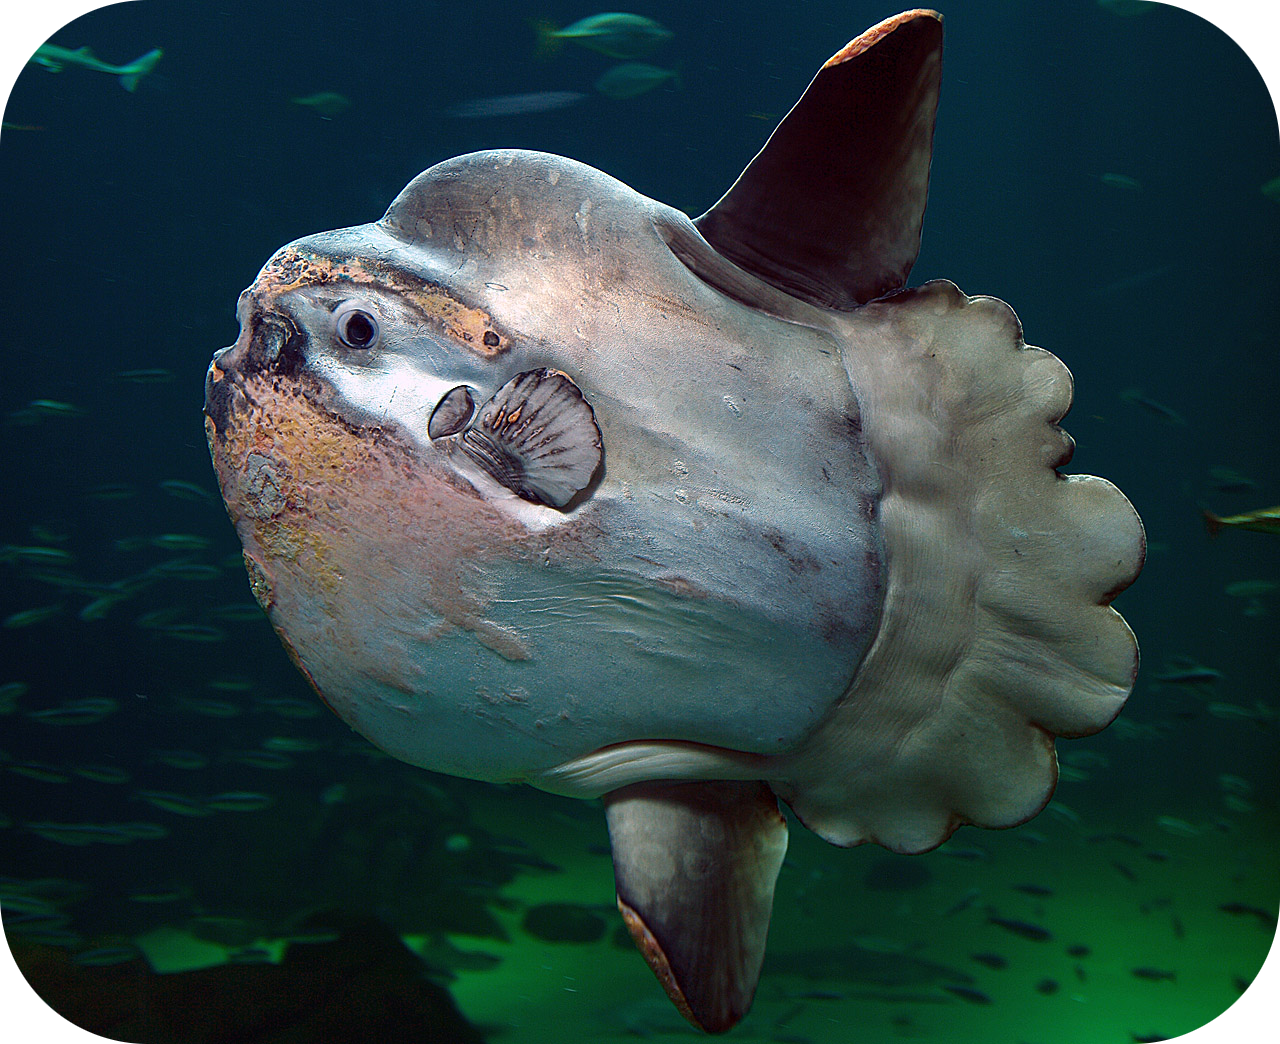
\includegraphics[height=.4\textheight]{molamola.png}
	\end{center}
}

%\titlegraphic{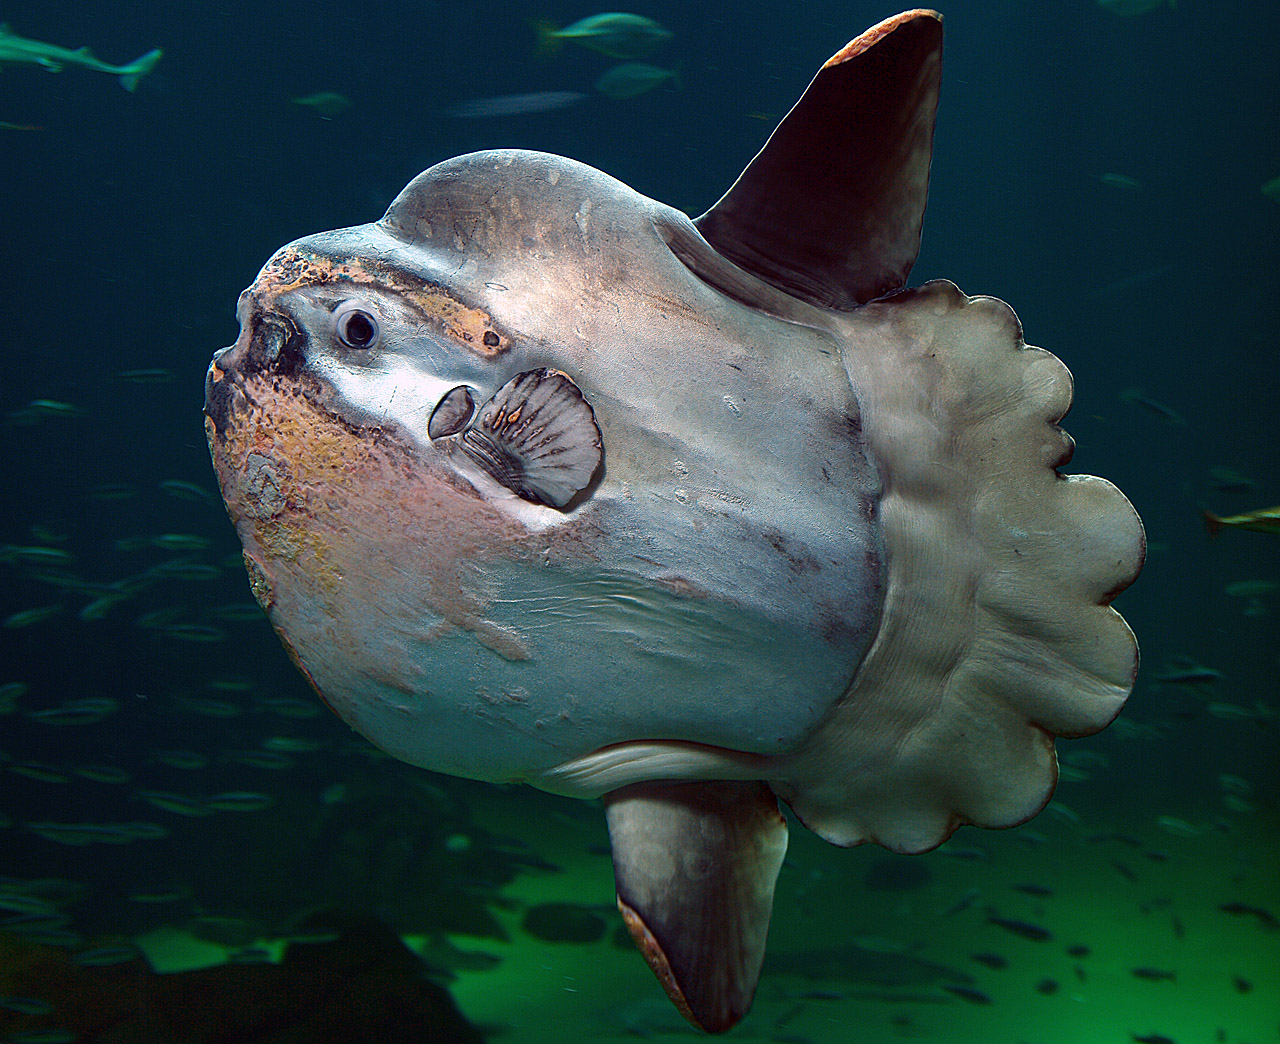
\includegraphics[width=\textwidth,height=.5\textheight]{molamola.jpg}}


\begin{document}

\maketitle

\begin{frame}{Le problème étudié}
	TODO: 3 slides + figures
	\bigskip
	\begin{columns}[T]
		\column{0.5\textwidth}
			\sectitle{Le problème}
			\begin{itemize}
				\item Reconaissance d'espèces marines et d'objets divers
				\item En temps réel :
				\begin{itemize}
					\item Détection (???????)
					\item Classification
					\item Apprentissage de nouvelles données
				\end{itemize}
			\end{itemize}
		
		\column{0.5\textwidth}
			\sectitle{Les aspects difficiles}
			\begin{itemize}
				\item Complexité des fonds marins
				\item Diversité des espèces
				\item Peu de données pour certaines classes
			\end{itemize}
	\end{columns}
	\begin{columns}
		\column{0.7\textwidth}
			\begin{center}
			\sectitle{Utilité pratique}
			\end{center}
			\begin{itemize}
				\item Sous-marins autonomes
				\item Etudes non-destructive des populations
				\item Faibles coûts
			\end{itemize}
	\end{columns}
\end{frame}

\begin{frame}{Données utilisée}
	\begin{center}
		\begin{tabular}{ |m{14em}|m{14em}| }
			\hline
			\textbf{Fish4Knowledge species (F4K)} & \textbf{Images depuis Google (G)}  \\
			\hline\smallskip
			23 espèces & 150 espèces \\
			\smallskip
			12 122 images à 25 par espèce & 10 images par espèce \\
			Autour de $100\times100$ pixels & $128\times128$ pixels \\
			\hline
		\end{tabular} \\
		\bigskip
		\sectitle{Sous-sets de données}
		Origine des données et nombre d'images par espèce : \\
		\medskip
		\begin{tabular}{ |m{6.5em}|m{6.5em}|m{6.5em}|m{6.5em}| }
			\hline
			\textbf{3 espèces} & \textbf{6 espèces} &  \textbf{23 espèces} &  \textbf{173 espèces}\\
			\hline\smallskip
			F4K & F4K & F4K & F4K + G \\
			3200 à 4000 & 148 à 4000 & 25 à 4000 & 10 \\
			\hline
		\end{tabular}
	\end{center}
\end{frame}

\begin{frame}{Implémentation}
	\begin{columns}
		\column{0.5\textwidth}
		% python + DML + theano + local CPU
		\begin{center}
			\sectitle{Modèles légers}
			\medskip
			
\includegraphics[height=1.5em]{python.png}\\\smallskip
			
\includegraphics[height=1.5em]{numpy.png}\\\smallskip
			\textbf{\Large DML} \\\smallskip
			
\includegraphics[height=1.5em]{theano.png} \\\smallskip
			CPU local
		\end{center}
		
		\column{0.5\textwidth}
		% python + tf.Keras + tensorflow + GPU
		\begin{center}
			\sectitle{Modèles lourds}
			\medskip
			
\includegraphics[height=1.5em]{python.png}\\\smallskip
			
\includegraphics[height=1.5em]{numpy.png}\\\smallskip
			
\includegraphics[height=1.5em]{keras.png} \\\smallskip
			
\includegraphics[height=1.5em]{tensorflow.png} \\\smallskip
			\raisebox{-.25\height}{
\includegraphics[height=1.5em]{colab.png}} (GPU)
		\end{center}
	\end{columns}
	\begin{center}
		\sectitle{Classification rapide avec K plus proche voisins}
		\medskip
		
\includegraphics[height=2.5em]{cpp.png}
	\end{center}
\end{frame}

\section{Premières méthodes de classification}

\begin{frame}{Distances euclidiennes}
	\begin{columns}[T]
		\column{0.5\textwidth}
		\sectitle{K plus proches voisins (KNN)}
		\begin{itemize}
			\item Dimension $30 000$
			\item Dépend de la position de l'objet sur l'image
		\end{itemize}
		
		\column{0.5\textwidth}
		\sectitle{Densité de couleurs}
		\begin{itemize}
			\item Dimension $3$
			\item Indépendant de la position de l'objet
		\end{itemize}
	\end{columns}
	
	\begin{center}
		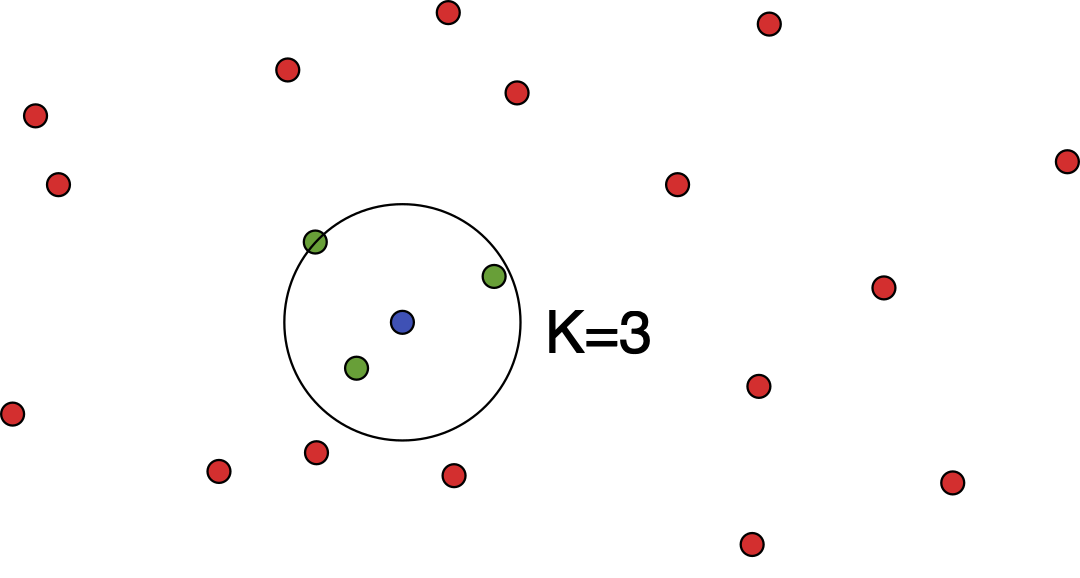
\includegraphics[width=.4\textwidth]{KNN.png}
		
		\begin{tabular}{ |m{6.5em}|m{6.5em}|m{6.5em}|m{6.5em}| }
			\hline
			& \textbf{3 espèces} & \textbf{6 espèces} &  \textbf{23 espèces} \\
			\hline\smallskip
			\textbf{KNN} & $91.6\%$ & $87.87\%$ & $38.84\%$ \\\smallskip
			\textbf{Densité} & $67.50\%$ & $39.73\%$ & $21.4\%$ \\\smallskip
			\textbf{Aléatoire} & $33.33\%$ & $16.67\%$ & $4.32\%$ \\
			\hline
		\end{tabular}
	\end{center}
	
	%\begin{theorem};
	%	Hey ! f(x)=42
	%\end{theorem}
\end{frame}

\begin{frame}{Construction d'un réseau de neurones (ANN)}
	\begin{block}{Ce qu'est réellement un ANN}
		Un réseau de neurones est une manière de représenter certaines fonctions non-linéaires
	\end{block}

	\begin{columns}
		\column{0.25\textwidth}
		\begin{flushright}
			\resizebox{4.5em}{!}{$\begin{pmatrix} a_{1}\\ a_{2}\\ \vdots \\ a_{n} \end{pmatrix}$}
		\end{flushright}
		\column{0.5\textwidth}
		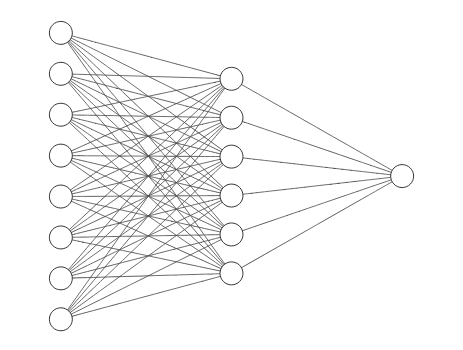
\includegraphics[width=\textwidth]{nnet.png}
		\column{0.25\textwidth}
		\resizebox{4em}{!}{$\begin{pmatrix} y_{1}\\ y_{2}\\ \vdots \\ y_{n} \end{pmatrix}$}
	\end{columns}
\end{frame}

\begin{frame}{Fonctionnement d'un neurone}
	\begin{center}
		\begin{tikzpicture}[x=0.75pt,y=0.75pt,yscale=-0.6,xscale=0.6]
		%uncomment if require: \path (0,300); %set diagram left start at 0, and has height of 300
		
		%Shape: Circle [id:dp22945892613165952] 
		\draw   (262,140.5) .. controls (262,104.88) and (290.88,76) .. (326.5,76) .. controls (362.12,76) and (391,104.88) .. (391,140.5) .. controls (391,176.12) and (362.12,205) .. (326.5,205) .. controls (290.88,205) and (262,176.12) .. (262,140.5) -- cycle ;
		%Straight Lines [id:da3910549433858823] 
		\draw    (99.5,141) -- (260,140.51) ;
		\draw [shift={(262,140.5)}, rotate = 539.8199999999999] [color={rgb, 255:red, 0; green, 0; blue, 0 }  ][line width=0.75]    (10.93,-3.29) .. controls (6.95,-1.4) and (3.31,-0.3) .. (0,0) .. controls (3.31,0.3) and (6.95,1.4) .. (10.93,3.29)   ;
		
		%Straight Lines [id:da0010243821676541032] 
		\draw    (99.5,200) -- (260.12,141.19) ;
		\draw [shift={(262,140.5)}, rotate = 519.89] [color={rgb, 255:red, 0; green, 0; blue, 0 }  ][line width=0.75]    (10.93,-3.29) .. controls (6.95,-1.4) and (3.31,-0.3) .. (0,0) .. controls (3.31,0.3) and (6.95,1.4) .. (10.93,3.29)   ;
		
		%Straight Lines [id:da3785492601580043] 
		\draw    (100.5,81) -- (260.12,139.81) ;
		\draw [shift={(262,140.5)}, rotate = 200.22] [color={rgb, 255:red, 0; green, 0; blue, 0 }  ][line width=0.75]    (10.93,-3.29) .. controls (6.95,-1.4) and (3.31,-0.3) .. (0,0) .. controls (3.31,0.3) and (6.95,1.4) .. (10.93,3.29)   ;
		
		%Straight Lines [id:da004064201434736736] 
		\draw  [dash pattern={on 0.84pt off 2.51pt}]  (103.5,34) -- (268.68,110.16) ;
		\draw [shift={(270.5,111)}, rotate = 204.75] [color={rgb, 255:red, 0; green, 0; blue, 0 }  ][line width=0.75]    (10.93,-3.29) .. controls (6.95,-1.4) and (3.31,-0.3) .. (0,0) .. controls (3.31,0.3) and (6.95,1.4) .. (10.93,3.29)   ;
		
		%Straight Lines [id:da36546984820866246] 
		\draw    (326.5,76) -- (326.5,205) ;
		
		
		%Straight Lines [id:da9555143146443819] 
		\draw    (391,140.5) -- (457.5,140.99) ;
		\draw [shift={(459.5,141)}, rotate = 180.42] [color={rgb, 255:red, 0; green, 0; blue, 0 }  ][line width=0.75]    (10.93,-3.29) .. controls (6.95,-1.4) and (3.31,-0.3) .. (0,0) .. controls (3.31,0.3) and (6.95,1.4) .. (10.93,3.29)   ;
		
		
		% Text Node
		\draw (79,80) node   {$a_{1}$};
		% Text Node
		\draw (80,140) node   {$a_{2}$};
		% Text Node
		\draw (81,199) node   {$a_{n}$};
		% Text Node
		\draw (167,88) node   {$w_{1}$};
		% Text Node
		\draw (165,125) node   {$w_{2}$};
		% Text Node
		\draw (165,161) node   {$w_{n}$};
		% Text Node
		\draw (176,48) node   {$b$};
		% Text Node
		\draw (299,140) node   {$z$};
		% Text Node
		\draw (357,143) node   {$\sigma(z)$};
		% Text Node
		\draw (422,124) node   {$y$};
		% Text Node
		\draw (81,170) node   {$\vdots $};
		\end{tikzpicture}
	\end{center}
	\begin{columns}
		\column{0.5\textwidth}
		$$
			z=b+\sum_{i=1}^na_i\times b_i
		$$
		\medskip
		$$
		y=\sigma(z)
		$$
		
		
		\column{0.5\textwidth}
		\arrayrulecolor{lightgray}
		\begin{tabular}{ |c|c| }
			\hline
			{\footnotesize Sigmoïde}  & {\footnotesize Tanh} \\
			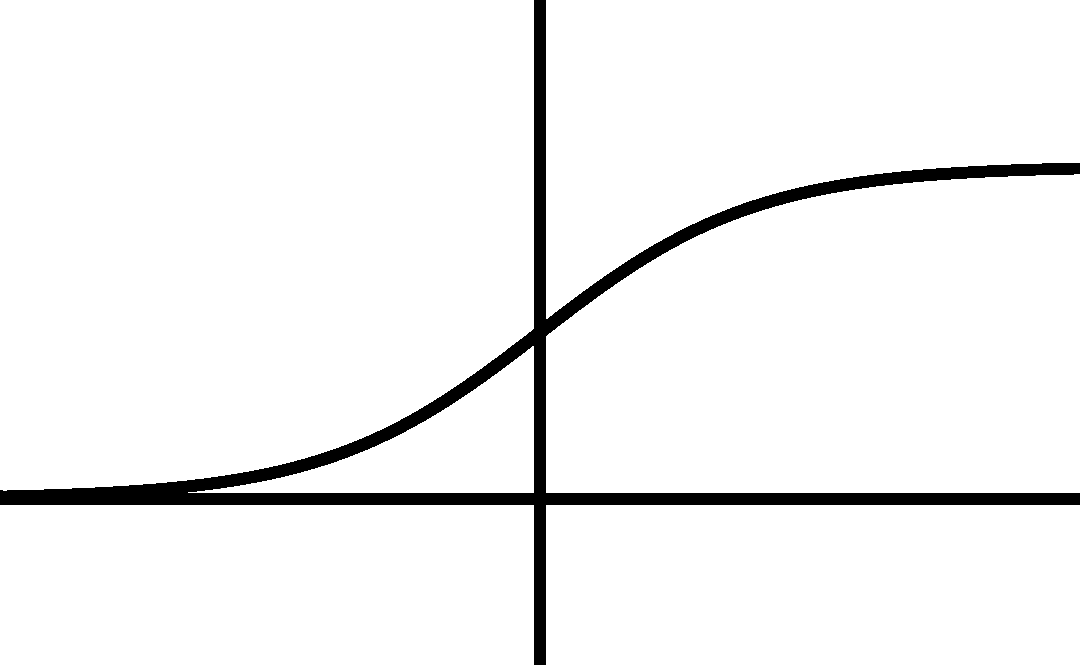
\includegraphics[width=5em]{sigmoid.png}& 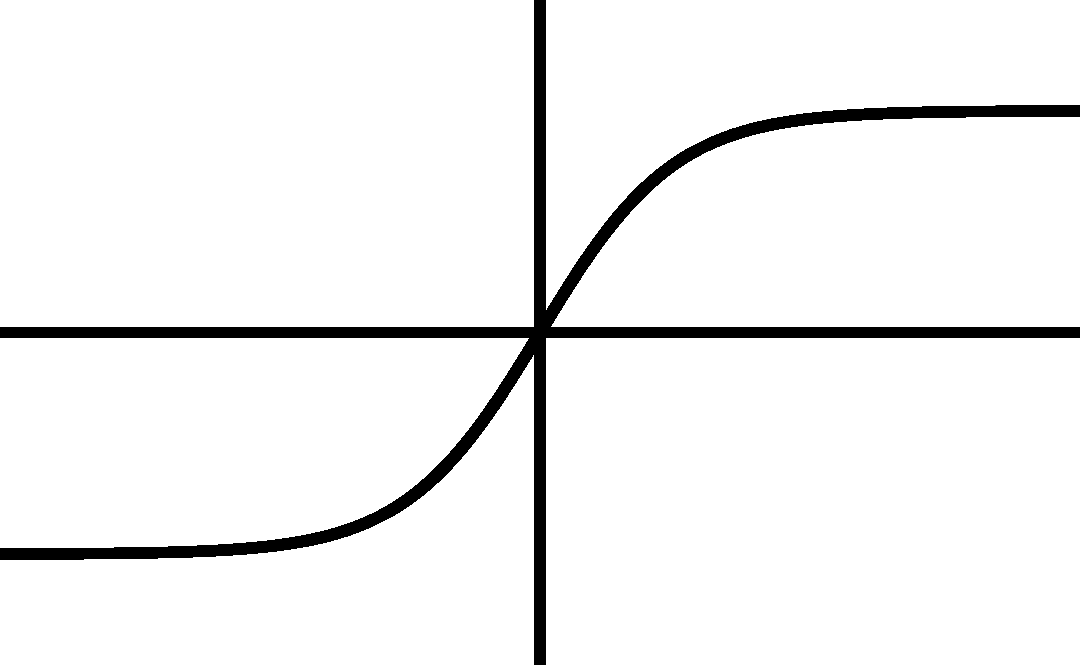
\includegraphics[width=5em]{tanh.png} \\
			$y=\frac{1}{1+e^{-z}}$ & $y=tanh(z)$ \\
			\hline
			{\footnotesize ReLU}  & {\footnotesize Weak ReLU} \\
			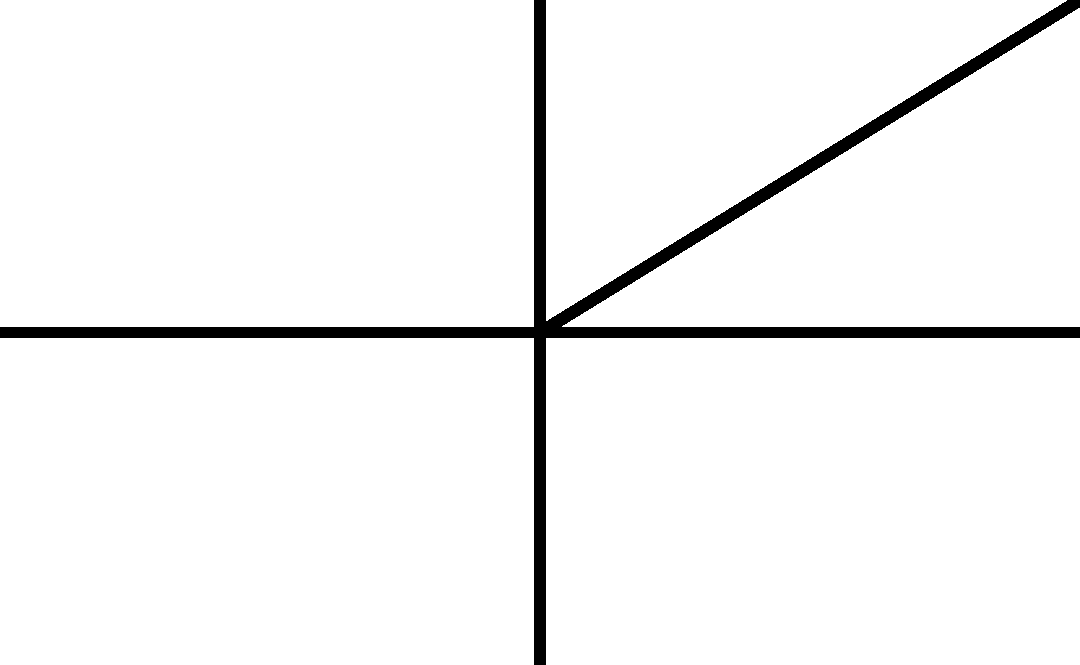
\includegraphics[width=5em]{relu.png}& 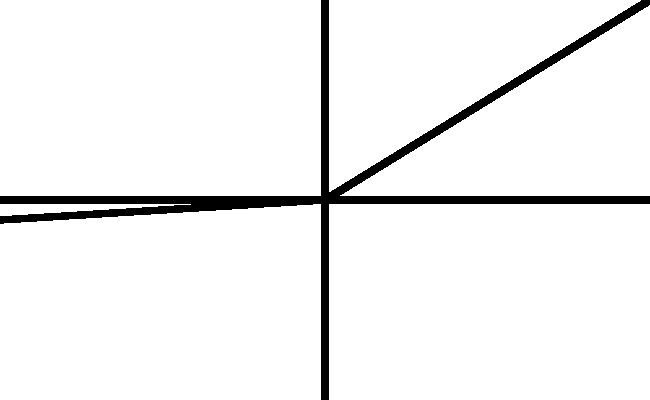
\includegraphics[width=5em]{weakrelu.png} \\
			$y=max(0,z)$ & $y=max(\epsilon\times z, z)$ \\
			\hline
		\end{tabular}
		\arrayrulecolor{black}
	\end{columns}
\end{frame}

\begin{frame}{Couche dense de neurones}
	\begin{columns}
		\column{0.3\textwidth}
		\begin{flushright}
			\resizebox{2em}{!}{$A^l$}
		\end{flushright}
		\column{0.4\textwidth}
		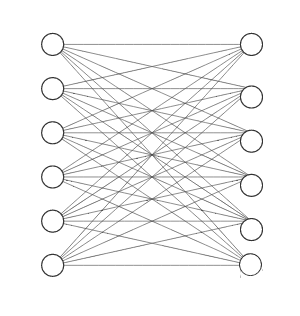
\includegraphics[width=\textwidth]{couche.png}
		\column{0.3\textwidth}
		\resizebox{2em}{!}{$Y^l$}
	\end{columns}
	\begin{columns}
		\column{0.3\textwidth}
		$$
		Z^l=W^l\times A^l+B^l
		$$
		$$
		Y^l=\sigma(Z^l)
		$$
		
		\column{0.3\textwidth}
		$$
			W=\begin{pmatrix} 
			w_{1,1} & \cdots &w_{1,n} \\
			w_{2,1} & \cdots &w_{2,n} \\
			\vdots & \ddots & \vdots \\
			w_{p,1} & \cdots &w_{p,n}
			\end{pmatrix}
		$$
		
		\column{0.3\textwidth}
		$$
			A=\begin{pmatrix}
			a_1 \\
			a_2 \\
			\vdots \\
			a_n
			\end{pmatrix}\ \ 
			B=\begin{pmatrix}
			b_1 \\
			b_2 \\
			\vdots \\
			b_p
			\end{pmatrix}
		$$
	\end{columns}
	\begin{center}
		$W^l$ et $B^l$ sont appris.
	\end{center}
	
\end{frame}

\begin{frame}{Entraînement}
	\begin{columns}[T]
		\column{0.5\textwidth}
		\sectitle{Fonction de coût $L_2$}
		$$
		C=\frac{1}{m}\sum_{i=1}^m (\hat{y}_i-y_i)^2
		$$
		Avec :
		\begin{itemize}
			\item $m$ : nombre d'images
			\item $\hat{y}$ : sortie attendue
		\end{itemize}
		\column{0.5\textwidth}
		\sectitle{Descente de gradient}
		$$
		W = W - \lambda \frac{\partial C}{\partial W}
		$$
		$$
		B = B - \lambda \frac{\partial C}{\partial B}
		$$
		{\centering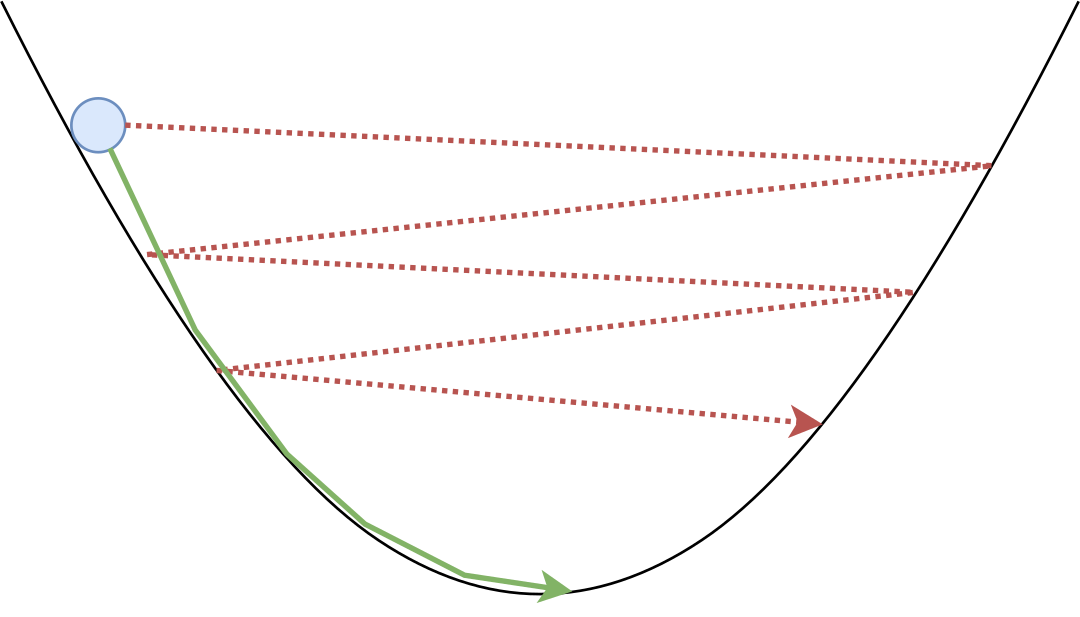
\includegraphics[width=\textwidth]{gradient.png}}
	\end{columns}
\end{frame}

\begin{frame}{Résultats intermédiaires 1}
	\begin{tabular}{ |m{10em}|m{5.5em}|m{5.5em}|m{5.5em}| }
		\hline
		Modèle & \textbf{3 espèces} & \textbf{6 espèces} &  \textbf{23 espèces} \\
		\hline
		\textbf{Aléatoire} & $33.33\%$ & $16.67\%$ & $4.32\%$ \\
		\textbf{KNN} & $91.6\%$ & $87.87\%$ & $38.84\%$ \\
		\textbf{ANN dense} & $96.83\%$ & $95.20\%$ & $83.58\%$ \\
		\hline
	\end{tabular}
	\begin{center}
	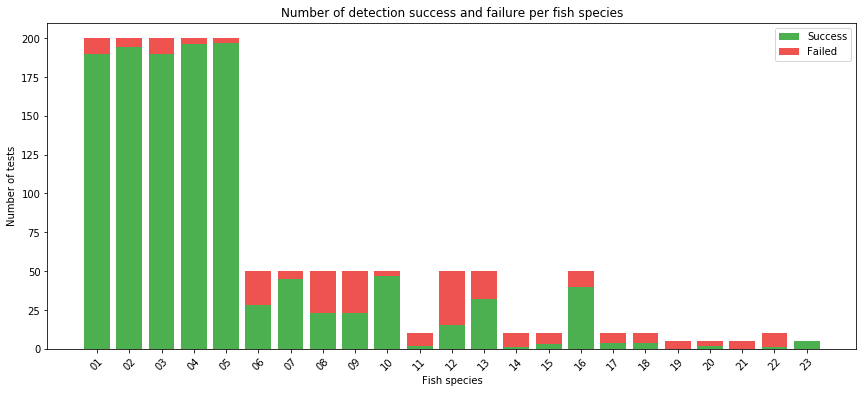
\includegraphics[width=\linewidth]{dense1_results.png}
	\end{center}
\end{frame}

\begin{frame}{Améliorer l'entrainement}
	\begin{columns}[T]
		\column{0.5\textwidth}
		\sectitle{Ajouter un moment au gradient}
		$$
		M_W=M_W - \lambda \frac{\partial C}{\partial W}
		$$
		$$
		W=W + M_W
		$$
		{\centering 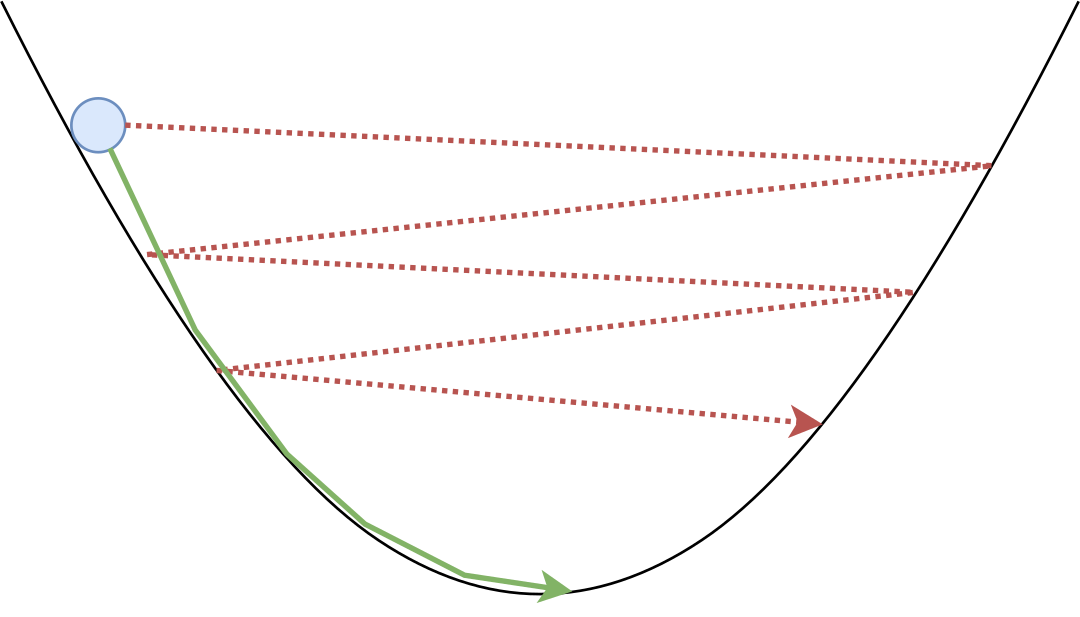
\includegraphics[width=0.9\textwidth]{gradient.png}}
		
		\column{0.5\textwidth}
		\sectitle{Couche softmax}
		Distribution de probabilité
		$$
		y^L_j=\frac{e^{z_j^L}}{\sum_i e^{z_i^L}}
		$$
		\medskip
		\textbf{Fonction de coût log-likelihood}
		$$
		C=-\log(y^L_{i_0})
		$$
		On a $\hat{y}$ de la forme $[0,\dots,0,1,0,\dots,0]$, et $\hat{y}_{i_0}=1$
		
	\end{columns}
\end{frame}

\begin{frame}{Normalisation}
	\begin{columns}[T]
		\column{0.45\textwidth}
		\sectitle{Entrées}
		$$
		\mu=\frac{1}{n}\sum_{i=1}^nX^{(i)}
		$$
		$$
		\sigma=\sqrt{\frac{1}{n}\sum_{i=1}^n(X^{(i)}-\mu)^2}
		$$
		
		Avec le carré élément par élément (au sens du produit de Hadamard).
		
		$$
		X^\prime=\frac{X-\mu}{\sigma}
		$$
		
		\column{0.55\textwidth}
		\sectitle{Activations}
		
		\begin{itemize}
			\item $\mu$ et $\sigma$ calculés par batchs
			\item $\alpha$ et $\beta$ paramètres appris
			\item $\gamma\in]0;1[$ fixe
		\end{itemize}
	
		{\centering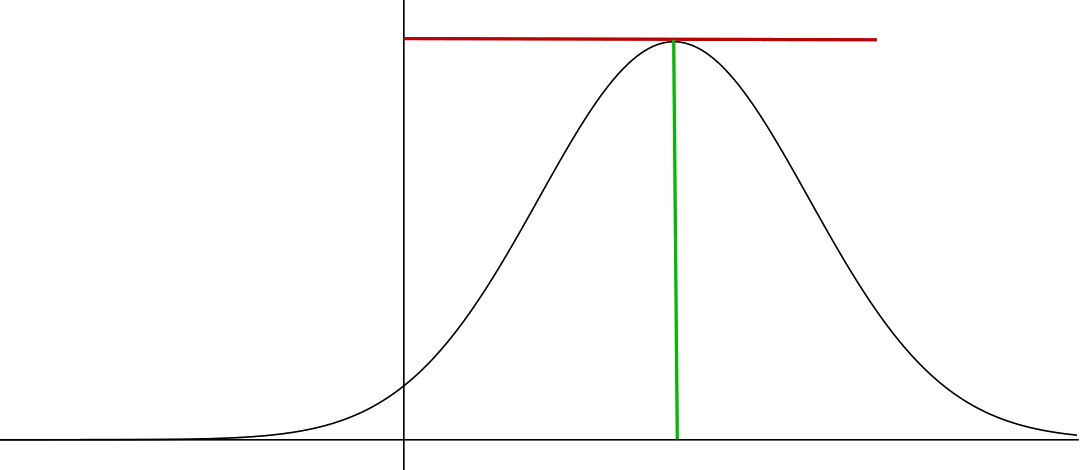
\includegraphics[width=0.8\textwidth]{gaussian.png}}
		
		
		$$
		\hat{\mu}=\gamma\hat{\mu}+(1-\gamma)\hat{\mu}
		\ \ \ \ \ \ \text{et} \ \ \ \ \ \ \hat{\sigma}=\gamma\hat{\sigma}+(1-\gamma)\hat{\sigma}
		$$
		
		$$
		a_{\text{norm}}=\alpha\frac{a-\hat{\mu}}{\hat{\sigma}}+\beta
		$$
	\end{columns}
\end{frame}

\begin{frame}{Résultats intermédiaires 2}
	\begin{tabular}{ |m{10em}|m{5.5em}|m{5.5em}|m{5.5em}| }
		\hline
		Modèle & \textbf{3 espèces} & \textbf{6 espèces} &  \textbf{23 espèces} \\
		\hline
		\textbf{Aléatoire} & $33.33\%$ & $16.67\%$ & $4.32\%$ \\
		\textbf{KNN} & $91.6\%$ & $87.87\%$ & $38.84\%$ \\
		\textbf{ANN dense} & $96.83\%$ & $95.20\%$ & $83.58\%$ \\
		\textbf{ANN dense amélioré} & $99.33\%$ & $95.60\%$ & $91.35\%$ \\
		\hline
	\end{tabular}
	\begin{center}
		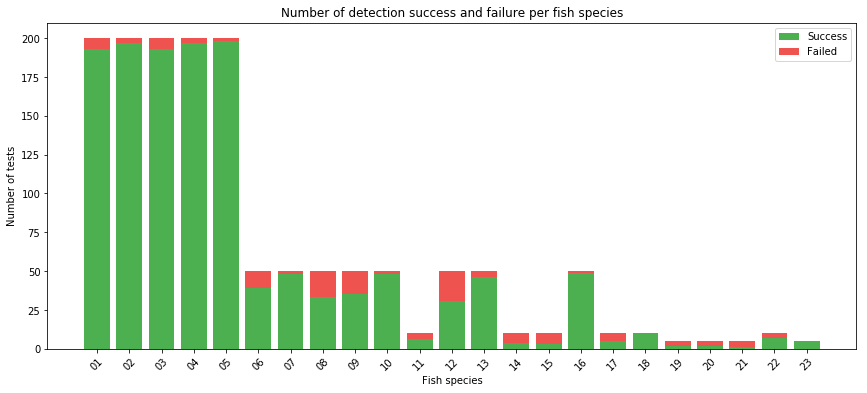
\includegraphics[width=\linewidth]{dense2_results.png}
	\end{center}
	
\end{frame}

\begin{frame}{Convolutions}
	Nouveau type de couche, utilisé pour créer un ConvNet. La matrice des filtres d'une couche sera une matrice 4D.
	\begin{center}
		\includegraphics[width=0.8\textwidth]{conv_net1.png}\\
		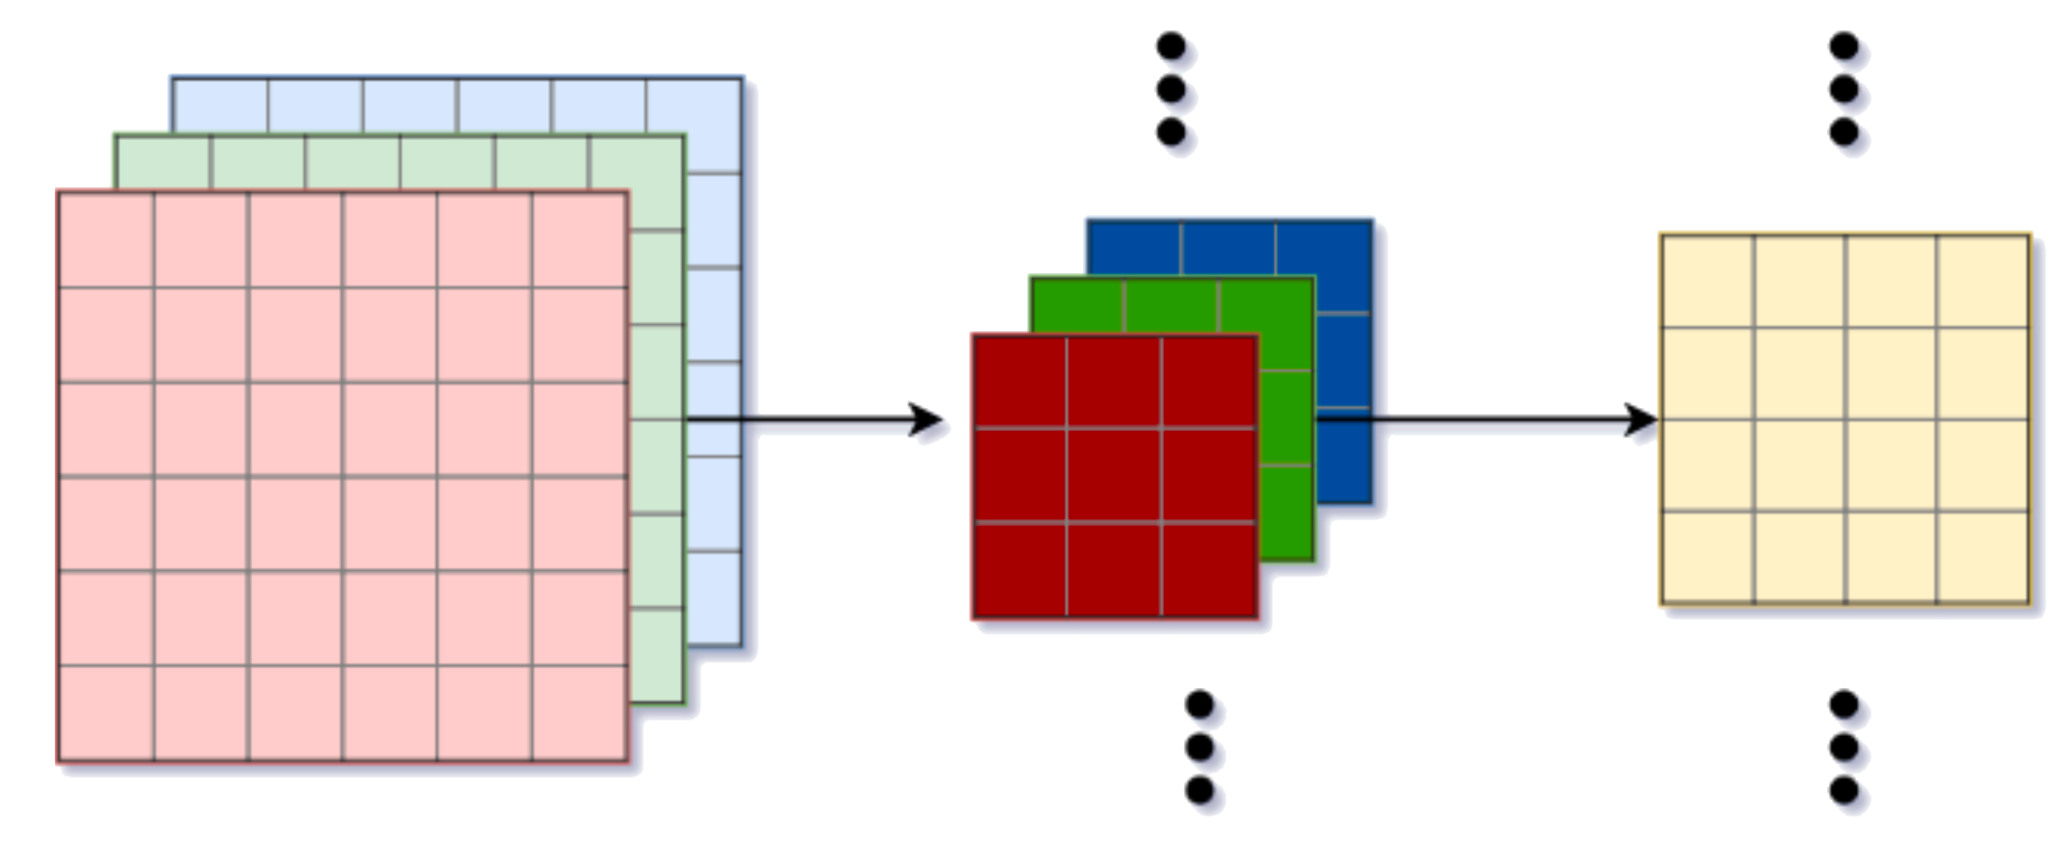
\includegraphics[width=0.7\textwidth]{conv_channels.png}
	\end{center}
\end{frame}

\begin{frame}{Pooling}
	Couche de max-pooling, suit une couche de convolution.
	\begin{center}
		\includegraphics[width=\textwidth]{maxpool.png}
	\end{center}
	Réduit la dimension spatiale et sélectionne l'information.
\end{frame}



\begin{frame}{Résultats intermédiaires 3}
	\begin{tabular}{ |m{10em}|m{5.5em}|m{5.5em}|m{5.5em}| }
		\hline
		Modèle & \textbf{3 espèces} & \textbf{6 espèces} &  \textbf{23 espèces} \\
		\hline
		\textbf{Aléatoire} & $33.33\%$ & $16.67\%$ & $4.32\%$ \\
		\textbf{KNN} & $91.6\%$ & $87.87\%$ & $38.84\%$ \\
		\textbf{ANN dense} & $96.83\%$ & $95.20\%$ & $83.58\%$ \\
		\textbf{ANN dense amélioré} & $99.33\%$ & $95.60\%$ & $91.35\%$ \\
		\textbf{ConvNet} & $99.50\%$ & $97.73\%$ & $96.96\%$ \\
		\hline
	\end{tabular}
	\begin{center}
		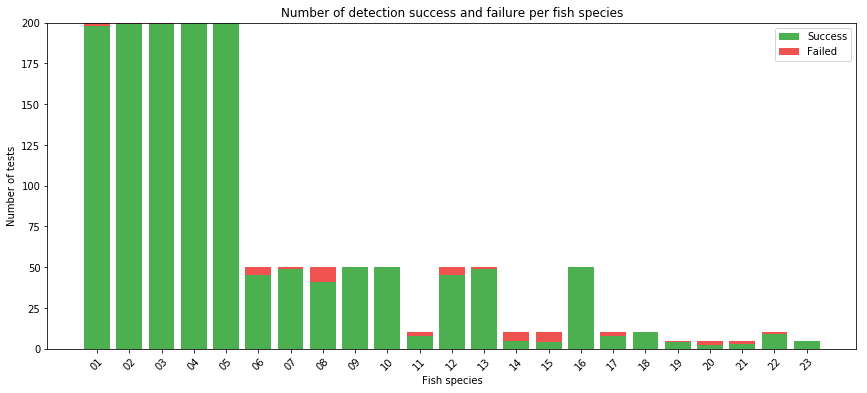
\includegraphics[width=\linewidth]{conv2_results.png}
	\end{center}
	
\end{frame}

\begin{frame}{Architectures}
	\begin{center}
		\sectitle{ANN dense}
		Paramètres : $102,787,095$\\
		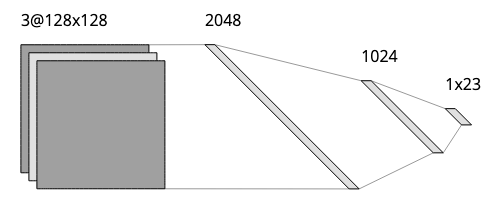
\includegraphics[width=0.66\textwidth]{dense_arch.png}
		\smallskip
		\newline
		\sectitle{ConvNet}
		Paramètres : $7,801,117$\\
		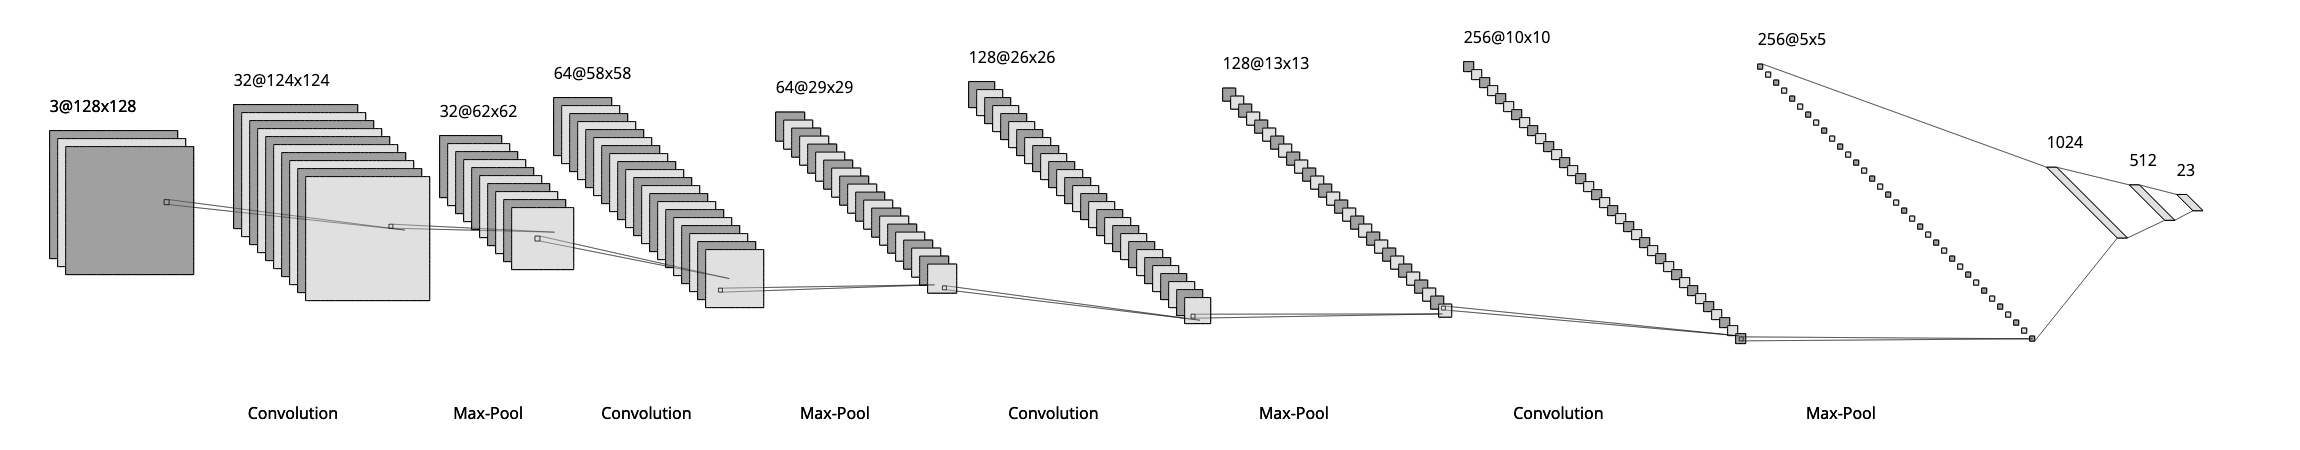
\includegraphics[width=1.1\textwidth]{conv2_arch.png}
	\end{center}
\end{frame}

\begin{frame}{Complexités}
	\begin{itemize}
		\item Pour une couche dense, $n$ et $m$ sont les tailles d'entrée et sortie
		\item Pour une couche de convolution :
		\begin{itemize}
			\item $n\times n\times m$ est la taille de l'entrée
			\item $k$ est la taille du filtre
			\item $l$ est le nombre de canaux de sortie
		\end{itemize}
	\end{itemize}
	\begin{center}
	\begin{tabular}{|c|c|}
		\hline
		\textbf{Opéation} & \textbf{Complexité} \\
		\hline
		Couche dense & $O(n\times m)$ \\
		\hline
		Convolution & $O(lmk^2n^2)$\\
		\hline
		Autres & $O(n)$\\
		\hline
	\end{tabular}
	\end{center}
\end{frame}

\begin{frame}{Limites}
	\begin{center}
		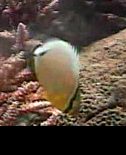
\includegraphics[width=4em]{fishes/5.png}
		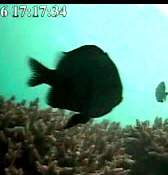
\includegraphics[width=4em]{fishes/1.png}
		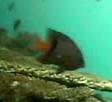
\includegraphics[width=4em]{fishes/2.png}
		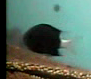
\includegraphics[width=4em]{fishes/3.png}
		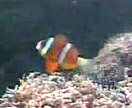
\includegraphics[width=4em]{fishes/4.png}
		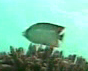
\includegraphics[width=4em]{fishes/6.png}
		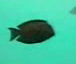
\includegraphics[width=4em]{fishes/8.png}
	\end{center}

	\begin{columns}
		\column{0.5\textwidth}
		\begin{itemize}
			\item Nombre de classes
			\item Temps d'entrainement :
			\begin{itemize}
				\item Ajout de données
				\item Ajout de classes
			\end{itemize}
		\end{itemize}
	\end{columns}

	\begin{center}
		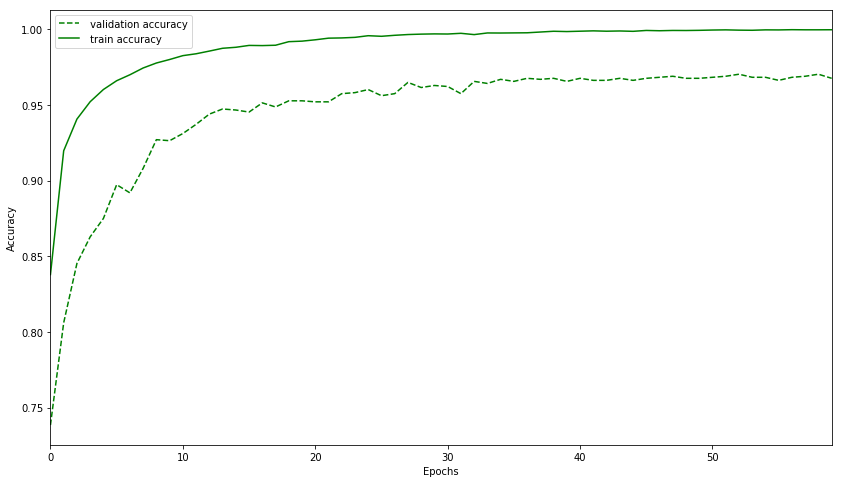
\includegraphics[width=12em]{train_3_acc.png}
		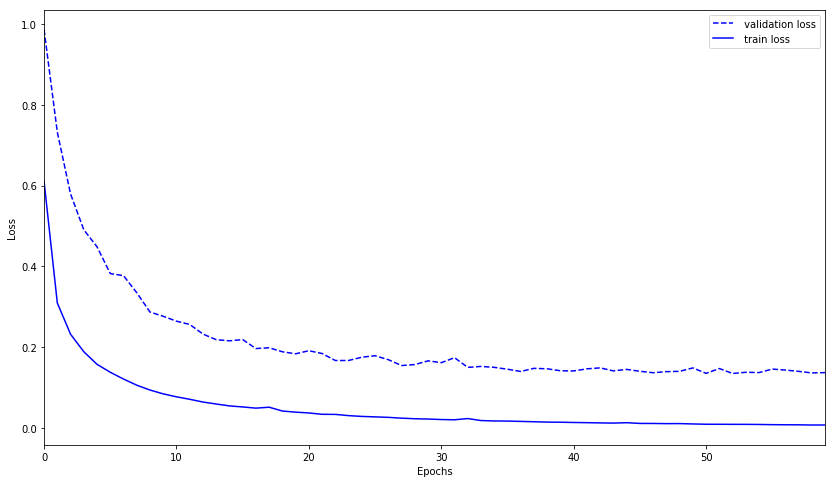
\includegraphics[width=12em]{train_3_loss.png}
	\end{center}
\end{frame}

\section{Transformation de l'image}

\begin{frame}{Ce que l'on cherche}
	\tikzset{every picture/.style={line width=0.75pt}} %set default line width to 0.75pt        
	
	\begin{tikzpicture}[x=0.75pt,y=0.75pt,yscale=-1,xscale=1]
	%uncomment if require: \path (0,400); %set diagram left start at 0, and has height of 400
	
	%Straight Lines [id:da2829187281066927] 
	\draw [line width=5.25]    (98.42,50.08) -- (188,52.76) ;
	\draw [shift={(196,53)}, rotate = 181.71] [fill={rgb, 255:red, 0; green, 0; blue, 0 }  ][line width=5.25]  [draw opacity=0] (29.47,-14.16) -- (0,0) -- (29.47,14.16) -- (19.57,0) -- cycle    ;
	
	\draw  [color={rgb, 255:red, 214; green, 34; blue, 34 }  ,draw opacity=1 ][line width=5.25]  (344.29,34.58) -- (372.61,65.57)(372.57,34.46) -- (344.33,65.7) ;
	%Straight Lines [id:da15738901895338753] 
	\draw [line width=5.25]    (99.88,84.99) -- (231.56,137.06) ;
	\draw [shift={(239,140)}, rotate = 201.57999999999998] [fill={rgb, 255:red, 0; green, 0; blue, 0 }  ][line width=5.25]  [draw opacity=0] (29.47,-14.16) -- (0,0) -- (29.47,14.16) -- (19.57,0) -- cycle    ;
	
	%Straight Lines [id:da7632009543226708] 
	\draw [line width=5.25]    (50.84,100.54) -- (50.84,164.45) ;
	\draw [shift={(50.84,172.45)}, rotate = 270] [fill={rgb, 255:red, 0; green, 0; blue, 0 }  ][line width=5.25]  [draw opacity=0] (29.47,-14.16) -- (0,0) -- (29.47,14.16) -- (19.57,0) -- cycle    ;
	
	\draw  [color={rgb, 255:red, 214; green, 34; blue, 34 }  ,draw opacity=1 ][line width=5.25]  (343.69,125.13) -- (372,156.12)(371.96,125.01) -- (343.72,156.24) ;
	%Image [id:dp3582590935616692] 
	\draw (50.84,52.29) node  {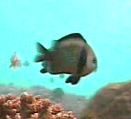
\includegraphics[width=56.75pt,height=58.19pt]{fish.png}};
	%Straight Lines [id:da03584674957949119] 
	\draw [color={rgb, 255:red, 43; green, 143; blue, 26 }  ,draw opacity=1 ][line width=4.5]    (107.77,220.31) -- (117.52,235.45) -- (135,208) ;
	
	
	
	% Text Node
	\draw (267.15,52.28) node [scale=0.7]  {$\begin{pmatrix}
		c_{1,1} & c_{1,2} & c_{1,3} & \dotsc  & c_{1,n}\\
		c_{2,1} & c_{2,2} & c_{2,3} & \dotsc  & c_{2,n}\\
		c_{3,1} & c_{3,2} & c_{3,3} & \dotsc  & c_{3,n}\\
		\vdots  & \vdots  & \vdots  & \ddots  & \vdots \\
		c_{n,1} & c_{n,2} & c_{n,3} & \dotsc  & c_{n,n}
		\end{pmatrix}$};
	% Text Node
	\draw (288.66,141.58) node   {$( R,V,B)$};
	% Text Node
	\draw (56,214.07) node   {$\begin{pmatrix}
		Carac\ 1\\
		Carac\ 2\\
		\vdots \\
		Carac\ m
		\end{pmatrix}$};
	% Text Node
	\draw (129.11,155.49) node [scale=1]  {$f:\mathbb{R}^{n\times n\times 3} \mapsto \mathbb{R}^{m}$};
	% Text Node
	\draw (221.48,223.37) node  [align=left] {Invariance selon la\\rotation, le fond, etc...};
	
	
	\end{tikzpicture}
	
\end{frame}

\begin{frame}{Réseau siamois}
	\begin{center}
		\begin{tikzpicture}[x=0.75pt,y=0.75pt,yscale=-1,xscale=1]
		%uncomment if require: \path (0,130); %set diagram left start at 0, and has height of 130
		
		%Image [id:dp5211780256446827] 
		\draw (40,47) node  {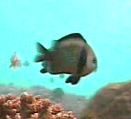
\includegraphics[width=42pt,height=43.5pt]{fish.png}};
		%Straight Lines [id:da5421577602072642] 
		\draw [line width=2.25]    (76,47) -- (99,47) ;
		\draw [shift={(103,47)}, rotate = 180] [fill={rgb, 255:red, 0; green, 0; blue, 0 }  ][line width=2.25]  [draw opacity=0] (14.29,-6.86) -- (0,0) -- (14.29,6.86) -- cycle    ;
		
		%Image [id:dp8003992435759841] 
		\draw (141,50) node  {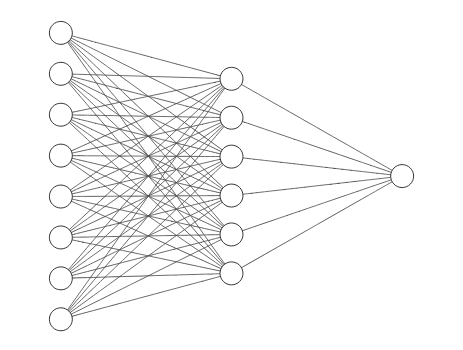
\includegraphics[width=52.5pt,height=52.5pt]{nnet.png}};
		%Straight Lines [id:da08283854498851895] 
		\draw [line width=2.25]    (179,51) -- (202,51) ;
		\draw [shift={(206,51)}, rotate = 180] [fill={rgb, 255:red, 0; green, 0; blue, 0 }  ][line width=2.25]  [draw opacity=0] (14.29,-6.86) -- (0,0) -- (14.29,6.86) -- cycle    ;
		
		
		% Text Node
		\draw (232,45) node [scale=0.8]  {$\begin{pmatrix}
			c_{1}\\
			c_{2}\\
			\vdots \\
			c_{m}
			\end{pmatrix}$};
		% Text Node
		\draw (130,104) node   {$f$};
		% Text Node
		\draw (233,106) node   {$f( a)$};
		% Text Node
		\draw (37,102) node   {$a$};
		
		
		\end{tikzpicture}
		
		\begin{tikzpicture}[x=0.75pt,y=0.75pt,yscale=-1,xscale=1]
		%uncomment if require: \path (0,159); %set diagram left start at 0, and has height of 159
		
		%Image [id:dp7928444210092973] 
		\draw (40,47) node  {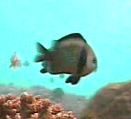
\includegraphics[width=42pt,height=43.5pt]{fish.png}};
		%Straight Lines [id:da05878974751078081] 
		\draw [line width=2.25]    (76,47) -- (99,47) ;
		\draw [shift={(103,47)}, rotate = 180] [fill={rgb, 255:red, 0; green, 0; blue, 0 }  ][line width=2.25]  [draw opacity=0] (14.29,-6.86) -- (0,0) -- (14.29,6.86) -- cycle    ;
		
		%Image [id:dp12389145525998724] 
		\draw (141,50) node  {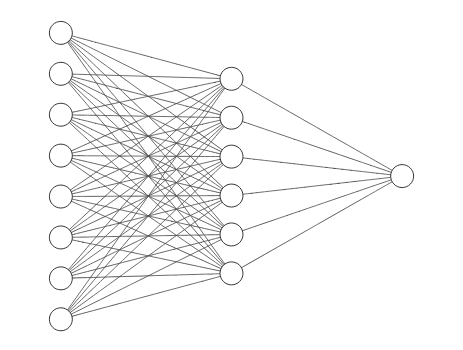
\includegraphics[width=52.5pt,height=52.5pt]{nnet.png}};
		%Straight Lines [id:da7699774306505847] 
		\draw [line width=2.25]    (79,123) -- (102,123) ;
		\draw [shift={(106,123)}, rotate = 180] [fill={rgb, 255:red, 0; green, 0; blue, 0 }  ][line width=2.25]  [draw opacity=0] (14.29,-6.86) -- (0,0) -- (14.29,6.86) -- cycle    ;
		
		%Image [id:dp4578141932551969] 
		\draw (41.5,120.5) node  {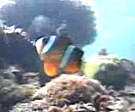
\includegraphics[width=42.75pt,height=39.75pt]{fish2.png}};
		%Image [id:dp034989969288212075] 
		\draw (141,120) node  {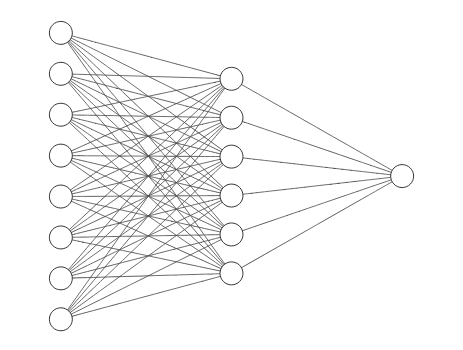
\includegraphics[width=52.5pt,height=52.5pt]{nnet.png}};
		%Straight Lines [id:da538314914281343] 
		\draw [line width=2.25]    (171,49) -- (201.17,79.17) ;
		\draw [shift={(204,82)}, rotate = 225] [fill={rgb, 255:red, 0; green, 0; blue, 0 }  ][line width=2.25]  [draw opacity=0] (14.29,-6.86) -- (0,0) -- (14.29,6.86) -- cycle    ;
		
		%Straight Lines [id:da7342166207918868] 
		\draw [line width=2.25]    (172,121) -- (200.13,93.78) ;
		\draw [shift={(203,91)}, rotate = 495.94] [fill={rgb, 255:red, 0; green, 0; blue, 0 }  ][line width=2.25]  [draw opacity=0] (14.29,-6.86) -- (0,0) -- (14.29,6.86) -- cycle    ;
		
		
		% Text Node
		\draw (238,123) node   {$=| f( b) -f( a)| $};
		% Text Node
		\draw (239,87) node   {$d( a,b)$};
		
		
		\end{tikzpicture}
		
	\end{center}

	
\end{frame}

\begin{frame}{Fonction de coût avec triplets}
	\begin{center}
		\begin{tikzpicture}[x=0.75pt,y=0.75pt,yscale=-1,xscale=1]
		%uncomment if require: \path (0,300); %set diagram left start at 0, and has height of 300
		
		%Image [id:dp06447046117833977] 
		\draw (46.5,44.5) node  {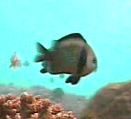
\includegraphics[width=50.25pt,height=53.25pt]{fish.png}};
		%Image [id:dp2844434061799066] 
		\draw (217,47) node  {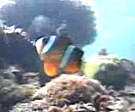
\includegraphics[width=52.5pt,height=52.5pt]{fish2.png}};
		%Image [id:dp531377260754192] 
		\draw (130,47) node  {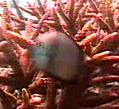
\includegraphics[width=52.5pt,height=52.5pt]{fish0.png}};
		
		% Text Node
		\draw (43,122) node   {$( ancre)$};
		% Text Node
		\draw (130,124) node   {$( positif)$};
		% Text Node
		\draw (216,124) node   {$( négatif)$};
		% Text Node
		\draw (40,97) node   {$a_{a}$};
		% Text Node
		\draw (124,98) node   {$a_{p}$};
		% Text Node
		\draw (215,97) node   {$a_{n}$};
		
		
		\end{tikzpicture}
		
	\end{center}
	On fixe la marge $m > 0$.
	$$
		C=max(0, d(a_a, a_p)-d(a_a, a_n))
	$$
\end{frame}

\begin{frame}{Sélectionner les triplets}
	
	\begin{center}
		\begin{tikzpicture}[x=0.75pt,y=0.75pt,yscale=-1,xscale=1]
		%uncomment if require: \path (0,300); %set diagram left start at 0, and has height of 300
		
		%Shape: Ellipse [id:dp1740239126512415] 
		\draw  [fill={rgb, 255:red, 216; green, 59; blue, 59 }  ,fill opacity=1 ] (58.53,37.11) .. controls (58.53,33.4) and (61.4,30.4) .. (64.93,30.4) .. controls (68.46,30.4) and (71.32,33.4) .. (71.32,37.11) .. controls (71.32,40.81) and (68.46,43.81) .. (64.93,43.81) .. controls (61.4,43.81) and (58.53,40.81) .. (58.53,37.11) -- cycle ;
		%Shape: Ellipse [id:dp8733584336558422] 
		\draw  [fill={rgb, 255:red, 216; green, 59; blue, 59 }  ,fill opacity=1 ] (86.96,66.92) .. controls (86.96,63.22) and (89.82,60.21) .. (93.35,60.21) .. controls (96.89,60.21) and (99.75,63.22) .. (99.75,66.92) .. controls (99.75,70.63) and (96.89,73.63) .. (93.35,73.63) .. controls (89.82,73.63) and (86.96,70.63) .. (86.96,66.92) -- cycle ;
		%Shape: Ellipse [id:dp9300236436471674] 
		\draw  [fill={rgb, 255:red, 216; green, 59; blue, 59 }  ,fill opacity=1 ] (58.53,65.43) .. controls (58.53,61.73) and (61.4,58.72) .. (64.93,58.72) .. controls (68.46,58.72) and (71.32,61.73) .. (71.32,65.43) .. controls (71.32,69.14) and (68.46,72.14) .. (64.93,72.14) .. controls (61.4,72.14) and (58.53,69.14) .. (58.53,65.43) -- cycle ;
		%Shape: Ellipse [id:dp178434239574375] 
		\draw  [fill={rgb, 255:red, 216; green, 59; blue, 59 }  ,fill opacity=1 ] (92.64,20.71) .. controls (92.64,17) and (95.51,14) .. (99.04,14) .. controls (102.57,14) and (105.44,17) .. (105.44,20.71) .. controls (105.44,24.41) and (102.57,27.42) .. (99.04,27.42) .. controls (95.51,27.42) and (92.64,24.41) .. (92.64,20.71) -- cycle ;
		%Shape: Ellipse [id:dp22113432762592677] 
		\draw  [fill={rgb, 255:red, 216; green, 59; blue, 59 }  ,fill opacity=1 ] (23,23.69) .. controls (23,19.98) and (25.86,16.98) .. (29.4,16.98) .. controls (32.93,16.98) and (35.79,19.98) .. (35.79,23.69) .. controls (35.79,27.39) and (32.93,30.4) .. (29.4,30.4) .. controls (25.86,30.4) and (23,27.39) .. (23,23.69) -- cycle ;
		%Shape: Ellipse [id:dp7533527732681178] 
		\draw  [fill={rgb, 255:red, 51; green, 122; blue, 202 }  ,fill opacity=1 ] (65.64,138.48) .. controls (65.64,134.77) and (68.5,131.77) .. (72.03,131.77) .. controls (75.57,131.77) and (78.43,134.77) .. (78.43,138.48) .. controls (78.43,142.18) and (75.57,145.19) .. (72.03,145.19) .. controls (68.5,145.19) and (65.64,142.18) .. (65.64,138.48) -- cycle ;
		%Shape: Ellipse [id:dp6543998872638248] 
		\draw  [fill={rgb, 255:red, 51; green, 122; blue, 202 }  ,fill opacity=1 ] (98.33,122.08) .. controls (98.33,118.37) and (101.19,115.37) .. (104.72,115.37) .. controls (108.26,115.37) and (111.12,118.37) .. (111.12,122.08) .. controls (111.12,125.78) and (108.26,128.79) .. (104.72,128.79) .. controls (101.19,128.79) and (98.33,125.78) .. (98.33,122.08) -- cycle ;
		%Shape: Ellipse [id:dp012910459910791205] 
		\draw  [fill={rgb, 255:red, 51; green, 122; blue, 202 }  ,fill opacity=1 ] (81.27,40.09) .. controls (81.27,36.38) and (84.14,33.38) .. (87.67,33.38) .. controls (91.2,33.38) and (94.06,36.38) .. (94.06,40.09) .. controls (94.06,43.79) and (91.2,46.8) .. (87.67,46.8) .. controls (84.14,46.8) and (81.27,43.79) .. (81.27,40.09) -- cycle ;
		%Shape: Ellipse [id:dp10884043431130741] 
		\draw  [fill={rgb, 255:red, 51; green, 122; blue, 202 }  ,fill opacity=1 ] (51.43,168.29) .. controls (51.43,164.59) and (54.29,161.58) .. (57.82,161.58) .. controls (61.35,161.58) and (64.22,164.59) .. (64.22,168.29) .. controls (64.22,172) and (61.35,175) .. (57.82,175) .. controls (54.29,175) and (51.43,172) .. (51.43,168.29) -- cycle ;
		%Shape: Ellipse [id:dp3518891652903833] 
		\draw  [fill={rgb, 255:red, 51; green, 122; blue, 202 }  ,fill opacity=1 ] (92.64,151.89) .. controls (92.64,148.19) and (95.51,145.19) .. (99.04,145.19) .. controls (102.57,145.19) and (105.44,148.19) .. (105.44,151.89) .. controls (105.44,155.6) and (102.57,158.6) .. (99.04,158.6) .. controls (95.51,158.6) and (92.64,155.6) .. (92.64,151.89) -- cycle ;
		%Shape: Ellipse [id:dp8683396909429699] 
		\draw  [fill={rgb, 255:red, 42; green, 151; blue, 24 }  ,fill opacity=1 ] (227.67,63.94) .. controls (227.67,60.23) and (230.53,57.23) .. (234.06,57.23) .. controls (237.59,57.23) and (240.46,60.23) .. (240.46,63.94) .. controls (240.46,67.64) and (237.59,70.65) .. (234.06,70.65) .. controls (230.53,70.65) and (227.67,67.64) .. (227.67,63.94) -- cycle ;
		%Shape: Ellipse [id:dp9683114563063726] 
		\draw  [fill={rgb, 255:red, 42; green, 151; blue, 24 }  ,fill opacity=1 ] (199.24,25.18) .. controls (199.24,21.48) and (202.1,18.47) .. (205.64,18.47) .. controls (209.17,18.47) and (212.03,21.48) .. (212.03,25.18) .. controls (212.03,28.89) and (209.17,31.89) .. (205.64,31.89) .. controls (202.1,31.89) and (199.24,28.89) .. (199.24,25.18) -- cycle ;
		%Shape: Ellipse [id:dp0425426292018265] 
		\draw  [fill={rgb, 255:red, 42; green, 151; blue, 24 }  ,fill opacity=1 ] (240.46,26.67) .. controls (240.46,22.97) and (243.32,19.96) .. (246.85,19.96) .. controls (250.39,19.96) and (253.25,22.97) .. (253.25,26.67) .. controls (253.25,30.38) and (250.39,33.38) .. (246.85,33.38) .. controls (243.32,33.38) and (240.46,30.38) .. (240.46,26.67) -- cycle ;
		%Shape: Ellipse [id:dp5949397558798495] 
		\draw  [fill={rgb, 255:red, 42; green, 151; blue, 24 }  ,fill opacity=1 ] (150.92,89.28) .. controls (150.92,85.58) and (153.78,82.57) .. (157.31,82.57) .. controls (160.84,82.57) and (163.71,85.58) .. (163.71,89.28) .. controls (163.71,92.99) and (160.84,95.99) .. (157.31,95.99) .. controls (153.78,95.99) and (150.92,92.99) .. (150.92,89.28) -- cycle ;
		%Shape: Ellipse [id:dp05454993749295367] 
		\draw  [fill={rgb, 255:red, 42; green, 151; blue, 24 }  ,fill opacity=1 ] (216.3,144.44) .. controls (216.3,140.73) and (219.16,137.73) .. (222.69,137.73) .. controls (226.22,137.73) and (229.09,140.73) .. (229.09,144.44) .. controls (229.09,148.14) and (226.22,151.15) .. (222.69,151.15) .. controls (219.16,151.15) and (216.3,148.14) .. (216.3,144.44) -- cycle ;
		%Shape: Ellipse [id:dp31383947975061544] 
		\draw  [fill={rgb, 255:red, 42; green, 151; blue, 24 }  ,fill opacity=1 ] (204.93,80.34) .. controls (204.93,76.63) and (207.79,73.63) .. (211.32,73.63) .. controls (214.85,73.63) and (217.72,76.63) .. (217.72,80.34) .. controls (217.72,84.04) and (214.85,87.05) .. (211.32,87.05) .. controls (207.79,87.05) and (204.93,84.04) .. (204.93,80.34) -- cycle ;
		%Shape: Ellipse [id:dp9237435667301697] 
		\draw  [fill={rgb, 255:red, 206; green, 221; blue, 31 }  ,fill opacity=1 ] (287.36,105.68) .. controls (287.36,101.98) and (290.22,98.97) .. (293.76,98.97) .. controls (297.29,98.97) and (300.15,101.98) .. (300.15,105.68) .. controls (300.15,109.39) and (297.29,112.39) .. (293.76,112.39) .. controls (290.22,112.39) and (287.36,109.39) .. (287.36,105.68) -- cycle ;
		%Shape: Ellipse [id:dp8431449554333157] 
		\draw  [fill={rgb, 255:red, 206; green, 221; blue, 31 }  ,fill opacity=1 ] (305.84,125.06) .. controls (305.84,121.36) and (308.7,118.35) .. (312.23,118.35) .. controls (315.77,118.35) and (318.63,121.36) .. (318.63,125.06) .. controls (318.63,128.77) and (315.77,131.77) .. (312.23,131.77) .. controls (308.7,131.77) and (305.84,128.77) .. (305.84,125.06) -- cycle ;
		%Shape: Ellipse [id:dp05913509228658875] 
		\draw  [fill={rgb, 255:red, 206; green, 221; blue, 31 }  ,fill opacity=1 ] (327.21,59) .. controls (327.21,55.29) and (330.07,52.29) .. (333.6,52.29) .. controls (337.14,52.29) and (340,55.29) .. (340,59) .. controls (340,62.7) and (337.14,65.7) .. (333.6,65.7) .. controls (330.07,65.7) and (327.21,62.7) .. (327.21,59) -- cycle ;
		%Shape: Ellipse [id:dp23645192909591173] 
		\draw  [fill={rgb, 255:red, 206; green, 221; blue, 31 }  ,fill opacity=1 ] (307.26,25.18) .. controls (307.26,21.48) and (310.12,18.47) .. (313.66,18.47) .. controls (317.19,18.47) and (320.05,21.48) .. (320.05,25.18) .. controls (320.05,28.89) and (317.19,31.89) .. (313.66,31.89) .. controls (310.12,31.89) and (307.26,28.89) .. (307.26,25.18) -- cycle ;
		%Shape: Ellipse [id:dp8885616715960105] 
		\draw  [fill={rgb, 255:red, 206; green, 221; blue, 31 }  ,fill opacity=1 ] (234.77,89.28) .. controls (234.77,85.58) and (237.64,82.57) .. (241.17,82.57) .. controls (244.7,82.57) and (247.56,85.58) .. (247.56,89.28) .. controls (247.56,92.99) and (244.7,95.99) .. (241.17,95.99) .. controls (237.64,95.99) and (234.77,92.99) .. (234.77,89.28) -- cycle ;
		\draw  [color={rgb, 255:red, 0; green, 0; blue, 0 }  ,draw opacity=1 ][line width=5.25]  (285.24,90.87) -- (312.64,64.94)(285.71,63.92) -- (312.18,91.89) ;
		\draw  [color={rgb, 255:red, 206; green, 221; blue, 31 }  ,draw opacity=1 ][line width=3.75]  (287.04,89.32) -- (311.13,66.52)(288.22,66.44) -- (309.95,89.4) ;
		%Straight Lines [id:da8520183169079636] 
		\draw  [dash pattern={on 4.5pt off 4.5pt}]  (313.66,25.18) -- (299,77) ;
		
		
		%Straight Lines [id:da03393581060138473] 
		\draw  [dash pattern={on 4.5pt off 4.5pt}]  (333.6,59) -- (299,77) ;
		
		
		%Straight Lines [id:da3611098067680698] 
		\draw  [dash pattern={on 4.5pt off 4.5pt}]  (312.23,125.06) -- (299,77) ;
		
		
		%Straight Lines [id:da21536454167746832] 
		\draw  [dash pattern={on 4.5pt off 4.5pt}]  (293.76,105.68) -- (299,77) ;
		
		
		%Straight Lines [id:da2563641465291293] 
		\draw  [dash pattern={on 4.5pt off 4.5pt}]  (299,77) -- (241.17,89.28) ;
		
		
		%Shape: Ellipse [id:dp3252041389011058] 
		\draw  [color={rgb, 255:red, 162; green, 17; blue, 17 }  ,draw opacity=1 ][line width=2.25]  (1.43,43.81) .. controls (1.43,22.28) and (29.86,4.81) .. (64.93,4.81) .. controls (100,4.81) and (128.43,22.28) .. (128.43,43.81) .. controls (128.43,65.35) and (100,82.81) .. (64.93,82.81) .. controls (29.86,82.81) and (1.43,65.35) .. (1.43,43.81) -- cycle ;
		%Shape: Ellipse [id:dp9471879975496891] 
		\draw  [color={rgb, 255:red, 30; green, 54; blue, 117 }  ,draw opacity=1 ][line width=2.25]  (14.93,143.74) .. controls (14.93,119.29) and (43.15,99.48) .. (77.97,99.48) .. controls (112.78,99.48) and (141,119.29) .. (141,143.74) .. controls (141,168.18) and (112.78,188) .. (77.97,188) .. controls (43.15,188) and (14.93,168.18) .. (14.93,143.74) -- cycle ;
		
		
		
		
		\end{tikzpicture}
		
	\end{center}
	
	\begin{block}{Algorithme rapide}
		- Un représentant par classe\\
		- Distance entre les représentants\\
		- Finalement, les 10 plus éloignés par image
	\end{block}

\end{frame}

\begin{frame}{Transfert d'apprentissage}
	\begin{center}
		\begin{tikzpicture}[x=0.75pt,y=0.75pt,yscale=-1,xscale=1]
		%uncomment if require: \path (0,300); %set diagram left start at 0, and has height of 300
		
		%Shape: Rectangle [id:dp08358039962974306] 
		\draw  [fill={rgb, 255:red, 1; green, 87; blue, 17 }  ,fill opacity=1 ] (10,11) -- (185,11) -- (185,109) -- (10,109) -- cycle ;
		%Shape: Rectangle [id:dp8005587326078292] 
		\draw  [fill={rgb, 255:red, 41; green, 61; blue, 190 }  ,fill opacity=1 ] (14,17) -- (121,17) -- (121,105) -- (14,105) -- cycle ;
		%Shape: Rectangle [id:dp8145151332573868] 
		\draw  [fill={rgb, 255:red, 31; green, 202; blue, 47 }  ,fill opacity=1 ] (128,17) -- (182,17) -- (182,105) -- (128,105) -- cycle ;
		%Shape: Rectangle [id:dp6058446903422545] 
		\draw  [fill={rgb, 255:red, 197; green, 68; blue, 68 }  ,fill opacity=1 ] (193,16) -- (242,16) -- (242,104) -- (193,104) -- cycle ;
		%Right Arrow [id:dp9277936351163816] 
		\draw  [fill={rgb, 255:red, 225; green, 241; blue, 31 }  ,fill opacity=1 ] (111,55) -- (128.4,55) -- (128.4,50) -- (140,60) -- (128.4,70) -- (128.4,65) -- (111,65) -- cycle ;
		%Right Arrow [id:dp42916714431721714] 
		\draw  [fill={rgb, 255:red, 225; green, 241; blue, 31 }  ,fill opacity=1 ] (173,55) -- (190.4,55) -- (190.4,50) -- (202,60) -- (190.4,70) -- (190.4,65) -- (173,65) -- cycle ;
		%Right Arrow [id:dp2285815434126115] 
		\draw  [fill={rgb, 255:red, 225; green, 241; blue, 31 }  ,fill opacity=1 ] (2,54) -- (19.4,54) -- (19.4,49) -- (31,59) -- (19.4,69) -- (19.4,64) -- (2,64) -- cycle ;
		%Right Arrow [id:dp3542152866659407] 
		\draw  [fill={rgb, 255:red, 225; green, 241; blue, 31 }  ,fill opacity=1 ] (232,58) -- (249.4,58) -- (249.4,53) -- (261,63) -- (249.4,73) -- (249.4,68) -- (232,68) -- cycle ;
		
		% Text Node
		\draw (99,150) node   {$\underbrace{\ \ \ \ \ \ \ \ \ \ \ \ \ \ \ \ \ \ \ \ \ \ \ \ \ \ \ \ \ \ \ \ \ \ \ \ \ \ \ \ \ \ }_{\text{Modèle pré-entrainé}}$};
		% Text Node
		\draw (157,128) node   {$\underbrace{\ \ \ \ \ \ \ \ \ \ \ \ }_{\text{Couches ré-entrainées}}$};
		% Text Node
		\draw (68,128) node   {$\underbrace{\ \ \ \ \ \ \ \ \ \ \ \ \ \ \ \ \ \ \ \ \ \ \ \ \ \ }_{\text{Couches gelées}}$};
		% Text Node
		\draw (219,116) node   {$\underbrace{\ \ \ \ \ \ \ \ \ \ }_{\text{Couches ajoutées}}$};
		
		\end{tikzpicture}
		\medskip
		\begin{columns}
			\column{0.5\textwidth}
			\sectitle{ConvNet}
			\begin{itemize}
				\item Entrainé sur F4K
				\item Spécialisé
				\item Ré-entrainé
			\end{itemize}
		
			\column{0.5\textwidth}
			\sectitle{MobileNet V2}
			\begin{itemize}
				\item Entrainé sur ImageNet
				\item Généraliste
				\item Utilisé tel quel
			\end{itemize}
		\end{columns}
		
	\end{center}
\end{frame}

\begin{frame}{Résultats}
	\begin{tabular}{ |m{10em}|m{8em}|m{8em}| }
		\hline
		Modèle & \textbf{173 espèces (entrainement)} & \textbf{23 espèces (test)} \\
		\hline
		\textbf{Aléatoire} & $0.58\%$ & $4.32\%$ \\
		\textbf{KNN} & $8.76\%$ & $38.8\%$ \\
		%\textbf{ConvNet} & - & $83.58\%$ \\
		\textbf{MobileNet + Siamois} & $26\%$ & $67\%$ \\
		\textbf{ConvNet + Siamois} & $91.85\%$ & $61.29\%$ \\
		\hline
	\end{tabular}
	\begin{center}
		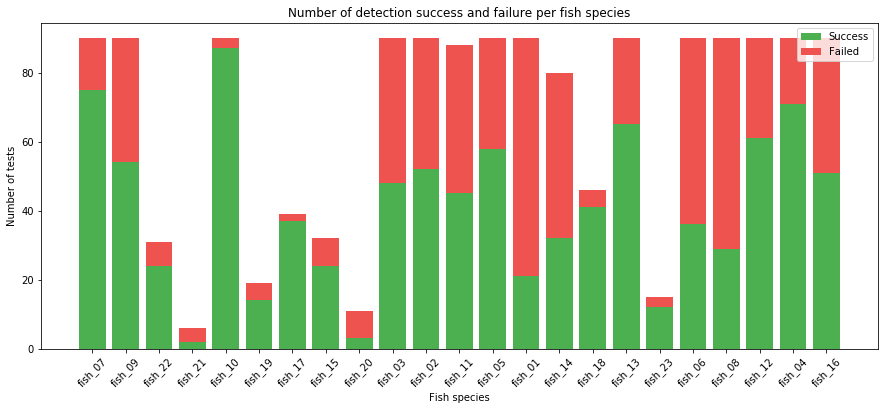
\includegraphics[width=\linewidth]{tl1_23out.png}
	\end{center}
\end{frame}

\begin{frame}{Statistiques sur l'entrainement}
	\begin{center}
		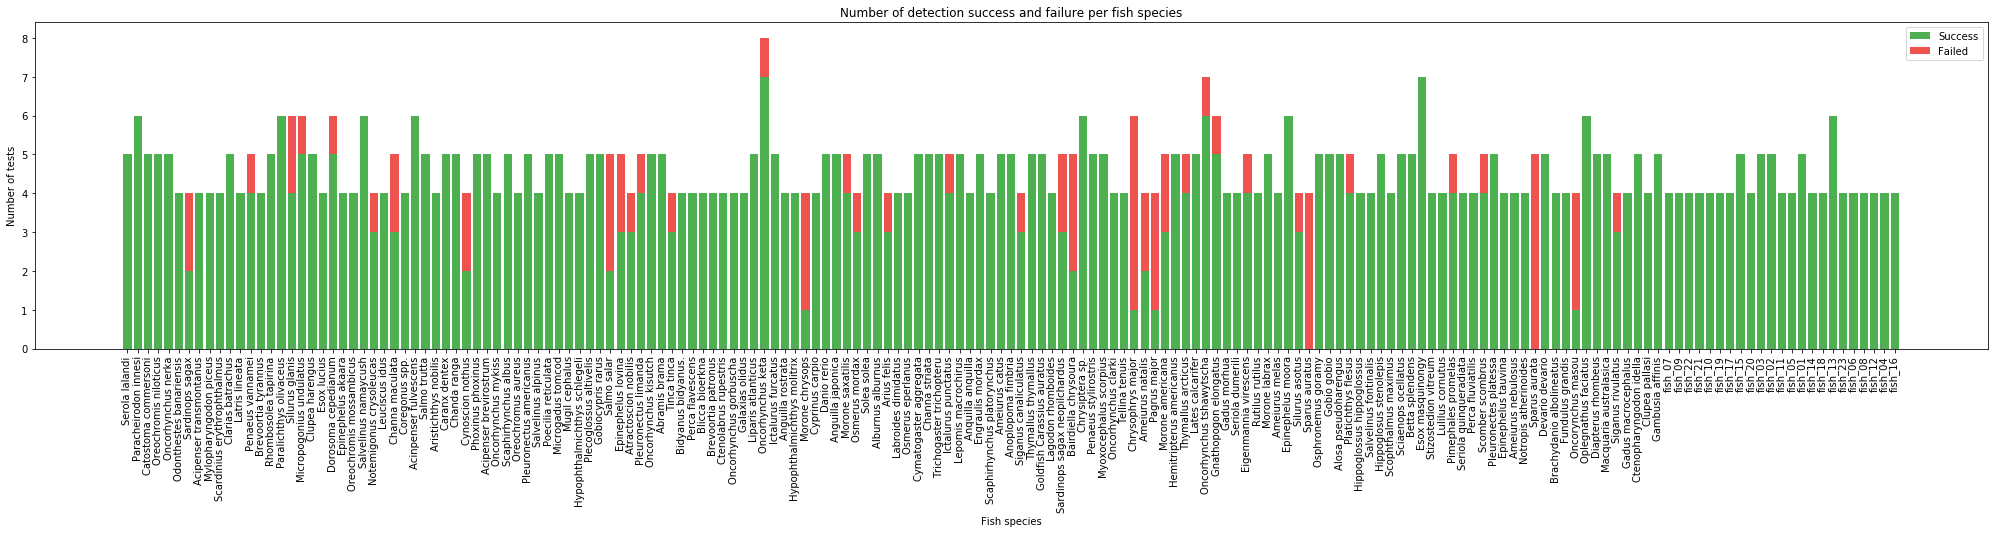
\includegraphics[width=30em,natwidth=1998,natheight=533]{stats1/tl1.2_150.png} \\
		\includegraphics[width=15em,natwidth=856,natheight=352]{stats1/tl1.2_150_repartition.png} \\
		\includegraphics[width=15em,natwidth=856,natheight=352]{stats1/same_repartition.png}
		\includegraphics[width=15em,natwidth=856,natheight=352]{stats1/tl1_23in_repartition.png}
	\end{center}
\end{frame}

\section{Classification rapide avec K plus proches voisins}

\begin{frame}{Problème des k plus proches en dimension quelconque}
		\begin{center}
		\begin{tikzpicture}[x=0.75pt,y=0.75pt,yscale=-1,xscale=1]
		%uncomment if require: \path (0,300); %set diagram left start at 0, and has height of 300
		
		%Shape: Circle [id:dp969964536191023] 
		\draw  [color={rgb, 255:red, 0; green, 121; blue, 21 }  ,draw opacity=1 ][fill={rgb, 255:red, 19; green, 187; blue, 46 }  ,fill opacity=0.28 ][line width=1.5]  (130.48,60.43) .. controls (130.48,37.8) and (148.82,19.46) .. (171.45,19.46) .. controls (194.07,19.46) and (212.41,37.8) .. (212.41,60.43) .. controls (212.41,83.05) and (194.07,101.39) .. (171.45,101.39) .. controls (148.82,101.39) and (130.48,83.05) .. (130.48,60.43) -- cycle ;
		%Shape: Ellipse [id:dp5180699511747047] 
		\draw  [fill={rgb, 255:red, 59; green, 139; blue, 216 }  ,fill opacity=1 ] (55.42,40.69) .. controls (55.42,36.73) and (58.44,33.52) .. (62.16,33.52) .. controls (65.88,33.52) and (68.89,36.73) .. (68.89,40.69) .. controls (68.89,44.64) and (65.88,47.85) .. (62.16,47.85) .. controls (58.44,47.85) and (55.42,44.64) .. (55.42,40.69) -- cycle ;
		%Shape: Ellipse [id:dp4937332850234284] 
		\draw  [fill={rgb, 255:red, 59; green, 139; blue, 216 }  ,fill opacity=1 ] (93.36,83.54) .. controls (93.36,79.58) and (96.37,76.37) .. (100.09,76.37) .. controls (103.81,76.37) and (106.83,79.58) .. (106.83,83.54) .. controls (106.83,87.5) and (103.81,90.7) .. (100.09,90.7) .. controls (96.37,90.7) and (93.36,87.5) .. (93.36,83.54) -- cycle ;
		%Shape: Ellipse [id:dp6982429362924976] 
		\draw  [fill={rgb, 255:red, 59; green, 139; blue, 216 }  ,fill opacity=1 ] (55.42,76.94) .. controls (55.42,72.99) and (58.44,69.78) .. (62.16,69.78) .. controls (65.88,69.78) and (68.89,72.99) .. (68.89,76.94) .. controls (68.89,80.9) and (65.88,84.11) .. (62.16,84.11) .. controls (58.44,84.11) and (55.42,80.9) .. (55.42,76.94) -- cycle ;
		%Shape: Ellipse [id:dp6893236026274245] 
		\draw  [fill={rgb, 255:red, 59; green, 139; blue, 216 }  ,fill opacity=1 ] (91.34,23.17) .. controls (91.34,19.21) and (94.36,16) .. (98.08,16) .. controls (101.8,16) and (104.81,19.21) .. (104.81,23.17) .. controls (104.81,27.12) and (101.8,30.33) .. (98.08,30.33) .. controls (94.36,30.33) and (91.34,27.12) .. (91.34,23.17) -- cycle ;
		%Shape: Ellipse [id:dp17709126318065138] 
		\draw  [fill={rgb, 255:red, 59; green, 139; blue, 216 }  ,fill opacity=1 ] (18,26.35) .. controls (18,22.39) and (21.02,19.19) .. (24.74,19.19) .. controls (28.46,19.19) and (31.47,22.39) .. (31.47,26.35) .. controls (31.47,30.31) and (28.46,33.52) .. (24.74,33.52) .. controls (21.02,33.52) and (18,30.31) .. (18,26.35) -- cycle ;
		%Shape: Ellipse [id:dp9614497921493588] 
		\draw  [fill={rgb, 255:red, 59; green, 139; blue, 216 }  ,fill opacity=1 ] (65.9,121.98) .. controls (65.9,118.02) and (68.92,114.81) .. (72.64,114.81) .. controls (76.36,114.81) and (79.38,118.02) .. (79.38,121.98) .. controls (79.38,125.94) and (76.36,129.15) .. (72.64,129.15) .. controls (68.92,129.15) and (65.9,125.94) .. (65.9,121.98) -- cycle ;
		%Shape: Ellipse [id:dp43683275050784953] 
		\draw  [fill={rgb, 255:red, 59; green, 139; blue, 216 }  ,fill opacity=1 ] (97.33,131.46) .. controls (97.33,127.5) and (100.35,124.3) .. (104.07,124.3) .. controls (107.79,124.3) and (110.8,127.5) .. (110.8,131.46) .. controls (110.8,135.42) and (107.79,138.63) .. (104.07,138.63) .. controls (100.35,138.63) and (97.33,135.42) .. (97.33,131.46) -- cycle ;
		%Shape: Ellipse [id:dp9106503058391959] 
		\draw  [fill={rgb, 255:red, 59; green, 139; blue, 216 }  ,fill opacity=1 ] (127.37,57.87) .. controls (127.37,53.91) and (130.38,50.7) .. (134.1,50.7) .. controls (137.82,50.7) and (140.84,53.91) .. (140.84,57.87) .. controls (140.84,61.83) and (137.82,65.04) .. (134.1,65.04) .. controls (130.38,65.04) and (127.37,61.83) .. (127.37,57.87) -- cycle ;
		%Shape: Ellipse [id:dp07337970484040479] 
		\draw  [fill={rgb, 255:red, 59; green, 139; blue, 216 }  ,fill opacity=1 ] (3.94,131.83) .. controls (3.94,127.88) and (6.95,124.67) .. (10.67,124.67) .. controls (14.39,124.67) and (17.41,127.88) .. (17.41,131.83) .. controls (17.41,135.79) and (14.39,139) .. (10.67,139) .. controls (6.95,139) and (3.94,135.79) .. (3.94,131.83) -- cycle ;
		%Shape: Ellipse [id:dp779475121007069] 
		\draw  [fill={rgb, 255:red, 59; green, 139; blue, 216 }  ,fill opacity=1 ] (169.34,157.31) .. controls (169.34,153.36) and (172.36,150.15) .. (176.08,150.15) .. controls (179.8,150.15) and (182.81,153.36) .. (182.81,157.31) .. controls (182.81,161.27) and (179.8,164.48) .. (176.08,164.48) .. controls (172.36,164.48) and (169.34,161.27) .. (169.34,157.31) -- cycle ;
		%Shape: Ellipse [id:dp023011662369415653] 
		\draw  [fill={rgb, 255:red, 59; green, 139; blue, 216 }  ,fill opacity=1 ] (233.54,69.35) .. controls (233.54,65.39) and (236.55,62.19) .. (240.27,62.19) .. controls (243.99,62.19) and (247.01,65.39) .. (247.01,69.35) .. controls (247.01,73.31) and (243.99,76.52) .. (240.27,76.52) .. controls (236.55,76.52) and (233.54,73.31) .. (233.54,69.35) -- cycle ;
		%Shape: Ellipse [id:dp23606121447182504] 
		\draw  [fill={rgb, 255:red, 59; green, 139; blue, 216 }  ,fill opacity=1 ] (191.6,29.94) .. controls (191.6,25.99) and (194.62,22.78) .. (198.34,22.78) .. controls (202.06,22.78) and (205.07,25.99) .. (205.07,29.94) .. controls (205.07,33.9) and (202.06,37.11) .. (198.34,37.11) .. controls (194.62,37.11) and (191.6,33.9) .. (191.6,29.94) -- cycle ;
		%Shape: Ellipse [id:dp21404207463271896] 
		\draw  [fill={rgb, 255:red, 59; green, 139; blue, 216 }  ,fill opacity=1 ] (247.01,29.54) .. controls (247.01,25.58) and (250.03,22.37) .. (253.75,22.37) .. controls (257.47,22.37) and (260.48,25.58) .. (260.48,29.54) .. controls (260.48,33.5) and (257.47,36.7) .. (253.75,36.7) .. controls (250.03,36.7) and (247.01,33.5) .. (247.01,29.54) -- cycle ;
		%Shape: Ellipse [id:dp25669995465958206] 
		\draw  [fill={rgb, 255:red, 59; green, 139; blue, 216 }  ,fill opacity=1 ] (151.71,83.43) .. controls (151.71,79.47) and (154.73,76.26) .. (158.45,76.26) .. controls (162.17,76.26) and (165.18,79.47) .. (165.18,83.43) .. controls (165.18,87.38) and (162.17,90.59) .. (158.45,90.59) .. controls (154.73,90.59) and (151.71,87.38) .. (151.71,83.43) -- cycle ;
		%Shape: Ellipse [id:dp0024324021709658528] 
		\draw  [fill={rgb, 255:red, 59; green, 139; blue, 216 }  ,fill opacity=1 ] (221.56,155.35) .. controls (221.56,151.39) and (224.58,148.19) .. (228.3,148.19) .. controls (232.02,148.19) and (235.04,151.39) .. (235.04,155.35) .. controls (235.04,159.31) and (232.02,162.52) .. (228.3,162.52) .. controls (224.58,162.52) and (221.56,159.31) .. (221.56,155.35) -- cycle ;
		%Shape: Ellipse [id:dp9576167706654921] 
		\draw  [fill={rgb, 255:red, 59; green, 139; blue, 216 }  ,fill opacity=1 ] (211.59,90.87) .. controls (211.59,86.91) and (214.61,83.7) .. (218.33,83.7) .. controls (222.05,83.7) and (225.06,86.91) .. (225.06,90.87) .. controls (225.06,94.83) and (222.05,98.04) .. (218.33,98.04) .. controls (214.61,98.04) and (211.59,94.83) .. (211.59,90.87) -- cycle ;
		%Shape: Ellipse [id:dp31594355653374007] 
		\draw  [fill={rgb, 255:red, 59; green, 139; blue, 216 }  ,fill opacity=1 ] (296.4,113.94) .. controls (296.4,109.99) and (299.42,106.78) .. (303.14,106.78) .. controls (306.86,106.78) and (309.88,109.99) .. (309.88,113.94) .. controls (309.88,117.9) and (306.86,121.11) .. (303.14,121.11) .. controls (299.42,121.11) and (296.4,117.9) .. (296.4,113.94) -- cycle ;
		%Shape: Ellipse [id:dp4055138537812675] 
		\draw  [fill={rgb, 255:red, 59; green, 139; blue, 216 }  ,fill opacity=1 ] (315.86,134.65) .. controls (315.86,130.69) and (318.88,127.48) .. (322.6,127.48) .. controls (326.32,127.48) and (329.33,130.69) .. (329.33,134.65) .. controls (329.33,138.61) and (326.32,141.81) .. (322.6,141.81) .. controls (318.88,141.81) and (315.86,138.61) .. (315.86,134.65) -- cycle ;
		%Shape: Ellipse [id:dp23671520301861415] 
		\draw  [fill={rgb, 255:red, 59; green, 139; blue, 216 }  ,fill opacity=1 ] (317.36,27.94) .. controls (317.36,23.99) and (320.38,20.78) .. (324.1,20.78) .. controls (327.82,20.78) and (330.83,23.99) .. (330.83,27.94) .. controls (330.83,31.9) and (327.82,35.11) .. (324.1,35.11) .. controls (320.38,35.11) and (317.36,31.9) .. (317.36,27.94) -- cycle ;
		%Shape: Ellipse [id:dp2605302454406768] 
		\draw  [fill={rgb, 255:red, 59; green, 139; blue, 216 }  ,fill opacity=1 ] (241.02,96.43) .. controls (241.02,92.47) and (244.04,89.26) .. (247.76,89.26) .. controls (251.48,89.26) and (254.49,92.47) .. (254.49,96.43) .. controls (254.49,100.38) and (251.48,103.59) .. (247.76,103.59) .. controls (244.04,103.59) and (241.02,100.38) .. (241.02,96.43) -- cycle ;
		%Shape: Ellipse [id:dp2015884370157468] 
		\draw  [fill={rgb, 255:red, 59; green, 139; blue, 216 }  ,fill opacity=1 ] (340.53,69.61) .. controls (340.53,65.65) and (343.54,62.44) .. (347.26,62.44) .. controls (350.98,62.44) and (354,65.65) .. (354,69.61) .. controls (354,73.57) and (350.98,76.78) .. (347.26,76.78) .. controls (343.54,76.78) and (340.53,73.57) .. (340.53,69.61) -- cycle ;
		%Shape: Ellipse [id:dp7059293166601479] 
		\draw  [fill={rgb, 255:red, 52; green, 194; blue, 34 }  ,fill opacity=1 ] (164.71,60.43) .. controls (164.71,56.47) and (167.73,53.26) .. (171.45,53.26) .. controls (175.17,53.26) and (178.18,56.47) .. (178.18,60.43) .. controls (178.18,64.38) and (175.17,67.59) .. (171.45,67.59) .. controls (167.73,67.59) and (164.71,64.38) .. (164.71,60.43) -- cycle ;
		%Straight Lines [id:da07764258803761037] 
		\draw  [dash pattern={on 4.5pt off 4.5pt}]  (134.1,57.87) -- (171.45,60.43) ;
		
		
		%Straight Lines [id:da5192970393186629] 
		\draw  [dash pattern={on 4.5pt off 4.5pt}]  (171.45,60.43) -- (198.34,29.94) ;
		
		
		%Straight Lines [id:da940213383783773] 
		\draw  [dash pattern={on 4.5pt off 4.5pt}]  (158.45,83.43) -- (171.45,60.43) ;
		
		\end{tikzpicture}
		\end{center}
		
		\begin{itemize}
			\item Nombre de dimensions : $d\in\mathbb{N}*$ ($d\in\{1,2,32\}$) (??)
			\item Nombre de points : $n\in\mathbb{N}*$ ($n\in\{10,10^2,10^3,10^4\}$) (??)
			\item Nombre de voisins : $k\in\mathbb{N}*$  ($k\in\{1,2,3,5\}$) (??)
		\end{itemize}
	\end{frame}

\begin{frame}{Approche par force brute}
	\begin{block}{Idée}
		Parcourir tous les points en maintenant les plus proches avec un tas.
	\end{block}

	Somes stats ???
	
	\begin{block}{Complexité}
			$O(n)$ si $k=1$, $O(n\ln(k))$ si $k>1$
	\end{block}
\end{frame}

\begin{frame}{K-d tree ($k=1$ uniquement)}
	%\begin{block}{Idée}
	%	Séparer récursivement les points par un hyperplan, puis rechercher avec un branch-and-bound.
	%\end{block}
	
	\begin{center}
		\begin{tikzpicture}[x=0.75pt,y=0.75pt,yscale=-1,xscale=1]
		%uncomment if require: \path (0,211); %set diagram left start at 0, and has height of 211
		
		%Straight Lines [id:da7079414455451427] 
		\draw [color={rgb, 255:red, 26; green, 35; blue, 173 }  ,draw opacity=1 ][line width=1.5]    (89,23) -- (0,23) ;
		
		
		%Straight Lines [id:da1949978400832899] 
		\draw [color={rgb, 255:red, 164; green, 173; blue, 26 }  ,draw opacity=1 ][line width=1.5]    (88,102) -- (88,-1) ;
		
		
		%Straight Lines [id:da4687321487191336] 
		\draw [color={rgb, 255:red, 164; green, 173; blue, 26 }  ,draw opacity=1 ][line width=1.5]    (70,160) -- (70.09,101.54) ;
		
		
		%Straight Lines [id:da7676749600350481] 
		\draw [color={rgb, 255:red, 164; green, 173; blue, 26 }  ,draw opacity=1 ][line width=1.5]    (193,158) -- (193.16,75.94) ;
		
		
		%Straight Lines [id:da4658775415344458] 
		\draw [color={rgb, 255:red, 164; green, 173; blue, 26 }  ,draw opacity=1 ][line width=1.5]    (216.16,75.69) -- (216,0) ;
		
		
		%Straight Lines [id:da5125797691412224] 
		\draw [color={rgb, 255:red, 204; green, 75; blue, 20 }  ,draw opacity=1 ][line width=1.5]    (263.08,74.17) -- (125,75) ;
		
		
		%Straight Lines [id:da13131104675083582] 
		\draw [color={rgb, 255:red, 204; green, 75; blue, 20 }  ,draw opacity=1 ][line width=1.5]    (129,101) -- (-1,101) ;
		
		
		%Straight Lines [id:da7217948417162781] 
		\draw [color={rgb, 255:red, 38; green, 179; blue, 66 }  ,draw opacity=1 ][line width=1.5]    (128.74,-0.98) -- (128.74,158.02) ;
		
		
		%Shape: Ellipse [id:dp5964903164274455] 
		\draw  [fill={rgb, 255:red, 59; green, 139; blue, 216 }  ,fill opacity=1 ] (209.42,34.69) .. controls (209.42,30.73) and (212.44,27.52) .. (216.16,27.52) .. controls (219.88,27.52) and (222.89,30.73) .. (222.89,34.69) .. controls (222.89,38.64) and (219.88,41.85) .. (216.16,41.85) .. controls (212.44,41.85) and (209.42,38.64) .. (209.42,34.69) -- cycle ;
		%Shape: Ellipse [id:dp012650700053879804] 
		\draw  [fill={rgb, 255:red, 59; green, 139; blue, 216 }  ,fill opacity=1 ] (63.36,142.54) .. controls (63.36,138.58) and (66.37,135.37) .. (70.09,135.37) .. controls (73.81,135.37) and (76.83,138.58) .. (76.83,142.54) .. controls (76.83,146.5) and (73.81,149.7) .. (70.09,149.7) .. controls (66.37,149.7) and (63.36,146.5) .. (63.36,142.54) -- cycle ;
		%Shape: Ellipse [id:dp846679480370228] 
		\draw  [fill={rgb, 255:red, 59; green, 139; blue, 216 }  ,fill opacity=1 ] (186.42,116.94) .. controls (186.42,112.99) and (189.44,109.78) .. (193.16,109.78) .. controls (196.88,109.78) and (199.89,112.99) .. (199.89,116.94) .. controls (199.89,120.9) and (196.88,124.11) .. (193.16,124.11) .. controls (189.44,124.11) and (186.42,120.9) .. (186.42,116.94) -- cycle ;
		%Shape: Ellipse [id:dp43632384584709594] 
		\draw  [fill={rgb, 255:red, 59; green, 139; blue, 216 }  ,fill opacity=1 ] (256.34,74.17) .. controls (256.34,70.21) and (259.36,67) .. (263.08,67) .. controls (266.8,67) and (269.81,70.21) .. (269.81,74.17) .. controls (269.81,78.12) and (266.8,81.33) .. (263.08,81.33) .. controls (259.36,81.33) and (256.34,78.12) .. (256.34,74.17) -- cycle ;
		%Shape: Ellipse [id:dp5539102827903832] 
		\draw  [fill={rgb, 255:red, 59; green, 139; blue, 216 }  ,fill opacity=1 ] (122,71.35) .. controls (122,67.39) and (125.02,64.19) .. (128.74,64.19) .. controls (132.46,64.19) and (135.47,67.39) .. (135.47,71.35) .. controls (135.47,75.31) and (132.46,78.52) .. (128.74,78.52) .. controls (125.02,78.52) and (122,75.31) .. (122,71.35) -- cycle ;
		%Shape: Ellipse [id:dp012136325889228416] 
		\draw  [fill={rgb, 255:red, 59; green, 139; blue, 216 }  ,fill opacity=1 ] (80.9,34.98) .. controls (80.9,31.02) and (83.92,27.81) .. (87.64,27.81) .. controls (91.36,27.81) and (94.38,31.02) .. (94.38,34.98) .. controls (94.38,38.94) and (91.36,42.15) .. (87.64,42.15) .. controls (83.92,42.15) and (80.9,38.94) .. (80.9,34.98) -- cycle ;
		%Shape: Ellipse [id:dp6463290338154468] 
		\draw  [fill={rgb, 255:red, 59; green, 139; blue, 216 }  ,fill opacity=1 ] (39.94,101.83) .. controls (39.94,97.88) and (42.95,94.67) .. (46.67,94.67) .. controls (50.39,94.67) and (53.41,97.88) .. (53.41,101.83) .. controls (53.41,105.79) and (50.39,109) .. (46.67,109) .. controls (42.95,109) and (39.94,105.79) .. (39.94,101.83) -- cycle ;
		%Shape: Ellipse [id:dp18646495077898884] 
		\draw  [fill={rgb, 255:red, 59; green, 139; blue, 216 }  ,fill opacity=1 ] (18.71,23.43) .. controls (18.71,19.47) and (21.73,16.26) .. (25.45,16.26) .. controls (29.17,16.26) and (32.18,19.47) .. (32.18,23.43) .. controls (32.18,27.38) and (29.17,30.59) .. (25.45,30.59) .. controls (21.73,30.59) and (18.71,27.38) .. (18.71,23.43) -- cycle ;
		
		
		
		
		\end{tikzpicture}
		
		\begin{tikzpicture}[x=0.75pt,y=0.75pt,yscale=-1,xscale=1]
		%uncomment if require: \path (0,94); %set diagram left start at 0, and has height of 94
		
		%Straight Lines [id:da697163132946379] 
		\draw [color={rgb, 255:red, 38; green, 179; blue, 66 }  ,draw opacity=1 ][line width=1.5]    (113,0) -- (113.02,83.33) ;
		
		
		%Straight Lines [id:da15861145810880184] 
		\draw [color={rgb, 255:red, 204; green, 75; blue, 20 }  ,draw opacity=1 ][line width=1.5]    (251.08,65.17) -- (113,66) ;
		
		
		%Shape: Ellipse [id:dp5143450801330047] 
		\draw  [fill={rgb, 255:red, 52; green, 194; blue, 34 }  ,fill opacity=1 ] (151.55,45.32) .. controls (151.55,41.36) and (154.57,38.15) .. (158.29,38.15) .. controls (162.01,38.15) and (165.03,41.36) .. (165.03,45.32) .. controls (165.03,49.28) and (162.01,52.49) .. (158.29,52.49) .. controls (154.57,52.49) and (151.55,49.28) .. (151.55,45.32) -- cycle ;
		%Straight Lines [id:da6283851665777622] 
		\draw [color={rgb, 255:red, 204; green, 75; blue, 20 }  ,draw opacity=1 ][line width=1.5]    (113.08,29.17) -- (21,29) ;
		
		
		%Shape: Circle [id:dp6133949027986172] 
		\draw  [color={rgb, 255:red, 32; green, 172; blue, 219 }  ,draw opacity=1 ] (126.61,45.32) .. controls (126.61,27.82) and (140.79,13.64) .. (158.29,13.64) .. controls (175.79,13.64) and (189.97,27.82) .. (189.97,45.32) .. controls (189.97,62.82) and (175.79,77) .. (158.29,77) .. controls (140.79,77) and (126.61,62.82) .. (126.61,45.32) -- cycle ;
		
		
		
		
		\end{tikzpicture}
		
	\end{center}
	
	
	%\begin{block}{Complexité}
	%	Probabiliste. De $O(\ln(m))$ à $O(n)$
	%\end{block}
\end{frame}

\begin{frame}{Autres méthodes}
	TODO : stats de vitesse ET de \% de réussite pour toutes les méthodes
\end{frame}

\begin{frame}{Résultats (lesquels ?)}
	$$
	k=1, d=2
	$$
	\begin{center}\begin{tabular}{ |m{8em}|m{3.5em}|m{3.5em}| }
		\hline
		Algo & $n=10^2$ & $n=10^3$\\
		\hline
		\textbf{Force brute} & $100\%$ & $100\%$ \\
		\hline
	\end{tabular}\end{center}
\end{frame}

\section{Conclusion}

\begin{frame}[standout]
	Fin
\end{frame}

\end{document}
